\documentclass[11pt,fleqn,a4paper]{book}

%%%%%%%%%%%%%%%%%%%%%%%%%%%%%%%%%%%%%%%%%
% The Legrand Orange Book
% Structural Definitions File
% Version 2.0 (9/2/15)
%
% Original author:
% Mathias Legrand (legrand.mathias@gmail.com) with modifications by:
% Vel (vel@latextemplates.com)
%
% This file has been downloaded from:
% http://www.LaTeXTemplates.com
%
% License:
% CC BY-NC-SA 3.0 (http://creativecommons.org/licenses/by-nc-sa/3.0/)
%
%%%%%%%%%%%%%%%%%%%%%%%%%%%%%%%%%%%%%%%%%

%----------------------------------------------------------------------------------------
%	VARIOUS REQUIRED PACKAGES AND CONFIGURATIONS
%----------------------------------------------------------------------------------------

\usepackage[top=3cm,bottom=3cm,left=3cm,right=3cm,headsep=10pt,a4paper]{geometry} % Page margins

\usepackage{graphicx} % Required for including pictures
\graphicspath{{img/}} % Specifies the directory where pictures are stored

\usepackage{titling} % Macros for title, author, etc
\usepackage{lipsum} % Inserts dummy text

\usepackage{tikz} % Required for drawing custom shapes

\usepackage[english,dutch]{babel} % English language/hyphenation
\usepackage{iflang}

\usepackage{enumitem} % Customize lists
\setlist{nolistsep} % Reduce spacing between bullet points and numbered lists

\usepackage{booktabs} % Required for nicer horizontal rules in tables

\usepackage{xcolor} % Required for specifying colors by name
\definecolor{maincolor}{RGB}{0,100,184} % Define the main color used for highlighting throughout the book

% Paragraph style: no indent, add space between paragraphs
\setlength{\parindent}{0em}
\setlength{\parskip}{1em}

%----------------------------------------------------------------------------------------
%	FONTS
%----------------------------------------------------------------------------------------

\usepackage{avant} % Use the Avantgarde font for headings
%\usepackage{times} % Use the Times font for headings
\usepackage{mathptmx} % Use the Adobe Times Roman as the default text font together with math symbols from the Sym­bol, Chancery and Com­puter Modern fonts
\usepackage{eurosym}

\usepackage{amsfonts}
\usepackage{amsmath}
\usepackage{amssymb}
\usepackage{textcomp}
\usepackage{wasysym}

\usepackage{microtype} % Slightly tweak font spacing for aesthetics
\usepackage[utf8]{inputenc} % Required for including letters with accents
\usepackage[T1]{fontenc} % Use 8-bit encoding that has 256 glyphs

%------------------------------------------------------------------------------
%	TITLE PAGE
%------------------------------------------------------------------------------

\newcommand{\thetitlepage}{%
\begingroup
\thispagestyle{empty}
\begin{tikzpicture}[remember picture,overlay]
\coordinate [below=12cm] (midpoint) at (current page.north);
\node at (current page.north west)
{\begin{tikzpicture}[remember picture,overlay]
\node[anchor=north west,inner sep=0pt] at (0,0) {
\includegraphics[width=\paperwidth]{background}}; % Background image
\draw[anchor=north] (midpoint) node [fill=maincolor,fill opacity=0,text=white,text opacity=1,inner sep=1cm]{\Huge\centering\bfseries\sffamily\parbox[c][][t]{\paperwidth}{\centering \thetitle\\[15pt] % Book title
{\Large \thedate}\\[20pt] % Subtitle
{\large \theauthor}}}; % Author name
\end{tikzpicture}};
\end{tikzpicture}
\vfill
\endgroup
}

%----------------------------------------------------------------------------------------
%	BIBLIOGRAPHY AND INDEX
%----------------------------------------------------------------------------------------

\usepackage[style=apa,backend=biber]{biblatex}
\usepackage{csquotes}
\DeclareLanguageMapping{dutch}{dutch-apa}
\addbibresource{bibliografie.bib} % BibTeX bibliography file
\defbibheading{bibempty}{}

\usepackage{calc} % For simpler calculation - used for spacing the index letter headings correctly
\usepackage{makeidx} % Required to make an index
\makeindex % Tells LaTeX to create the files required for indexing

%----------------------------------------------------------------------------------------
%	MAIN TABLE OF CONTENTS
%----------------------------------------------------------------------------------------

\usepackage{titletoc} % Required for manipulating the table of contents

\contentsmargin{0cm} % Removes the default margin

% Part text styling
\titlecontents{part}[0cm]
{\addvspace{20pt}\centering\large\bfseries}
{}
{}
{}

% Chapter text styling
\titlecontents{chapter}[1.25cm] % Indentation
{\addvspace{12pt}\large\sffamily\bfseries} % Spacing and font options for chapters
{\color{maincolor!60}\contentslabel[\Large\thecontentslabel]{1.25cm}\color{maincolor}} % Chapter number
{\color{maincolor}}
{\color{maincolor!60}\normalsize\;\titlerule*[.5pc]{.}\;\thecontentspage} % Page number

% Section text styling
\titlecontents{section}[1.25cm] % Indentation
{\addvspace{3pt}\sffamily\bfseries} % Spacing and font options for sections
{\contentslabel[\thecontentslabel]{1.25cm}} % Section number
{}
{\hfill\color{black}\thecontentspage} % Page number
[]

% Subsection text styling
\titlecontents{subsection}[1.25cm] % Indentation
{\addvspace{1pt}\sffamily\small} % Spacing and font options for subsections
{\contentslabel[\thecontentslabel]{1.25cm}} % Subsection number
{}
{\ \titlerule*[.5pc]{.}\;\thecontentspage} % Page number
[]

% List of figures
\titlecontents{figure}[0em]
{\addvspace{-5pt}\sffamily}
{\thecontentslabel\hspace*{1em}}
{}
{\ \titlerule*[.5pc]{.}\;\thecontentspage}
[]

% List of tables
\titlecontents{table}[0em]
{\addvspace{-5pt}\sffamily}
{\thecontentslabel\hspace*{1em}}
{}
{\ \titlerule*[.5pc]{.}\;\thecontentspage}
[]

%----------------------------------------------------------------------------------------
%	MINI TABLE OF CONTENTS IN PART HEADS
%----------------------------------------------------------------------------------------

% Chapter text styling
\titlecontents{lchapter}[0em] % Indenting
{\addvspace{15pt}\large\sffamily\bfseries} % Spacing and font options for chapters
{\color{maincolor}\contentslabel[\Large\thecontentslabel]{1.25cm}\color{maincolor}} % Chapter number
{}
{\color{maincolor}\normalsize\sffamily\bfseries\;\titlerule*[.5pc]{.}\;\thecontentspage} % Page number

% Section text styling
\titlecontents{lsection}[0em] % Indenting
{\sffamily\small} % Spacing and font options for sections
{\contentslabel[\thecontentslabel]{1.25cm}} % Section number
{}
{}

% Subsection text styling
\titlecontents{lsubsection}[.5em] % Indentation
{\normalfont\footnotesize\sffamily} % Font settings
{}
{}
{}

%----------------------------------------------------------------------------------------
%	PAGE HEADERS
%----------------------------------------------------------------------------------------

\usepackage{fancyhdr} % Required for header and footer configuration

\pagestyle{fancy}
\renewcommand{\chaptermark}[1]{\markboth{\sffamily\normalsize\bfseries\chaptername\ \thechapter.\ #1}{}} % Chapter text font settings
\renewcommand{\sectionmark}[1]{\markright{\sffamily\normalsize\thesection\hspace{5pt}#1}{}} % Section text font settings
\fancyhf{} \fancyhead[LE,RO]{\sffamily\normalsize\thepage} % Font setting for the page number in the header
\fancyhead[LO]{\rightmark} % Print the nearest section name on the left side of odd pages
\fancyhead[RE]{\leftmark} % Print the current chapter name on the right side of even pages
\renewcommand{\headrulewidth}{0.5pt} % Width of the rule under the header
\addtolength{\headheight}{2.5pt} % Increase the spacing around the header slightly
\renewcommand{\footrulewidth}{0pt} % Removes the rule in the footer
\fancypagestyle{plain}{\fancyhead{}\renewcommand{\headrulewidth}{0pt}} % Style for when a plain pagestyle is specified

% Removes the header from odd empty pages at the end of chapters
\makeatletter
\renewcommand{\cleardoublepage}{
\clearpage\ifodd\c@page\else
\hbox{}
\vspace*{\fill}
\thispagestyle{empty}
\newpage
\fi}

%----------------------------------------------------------------------------------------
%	THEOREM STYLES
%----------------------------------------------------------------------------------------

\usepackage{amsmath,amsfonts,amssymb,amsthm} % For math equations, theorems, symbols, etc

\newcommand{\intoo}[2]{\mathopen{]}#1\,;#2\mathclose{[}}
\newcommand{\ud}{\mathop{\mathrm{{}d}}\mathopen{}}
\newcommand{\intff}[2]{\mathopen{[}#1\,;#2\mathclose{]}}
\newtheorem{notation}{Notation}[chapter]

% Boxed/framed environments
\newtheoremstyle{maincolornumbox}% % Theorem style name
{0pt}% Space above
{0pt}% Space below
{\normalfont}% % Body font
{}% Indent amount
{\small\bf\sffamily\color{maincolor}}% % Theorem head font
{\;}% Punctuation after theorem head
{0.25em}% Space after theorem head
{\small\sffamily\color{maincolor}\thmname{#1}\nobreakspace\thmnumber{\@ifnotempty{#1}{}\@upn{#2}}% Theorem text (e.g. Theorem 2.1)
\thmnote{\nobreakspace\the\thm@notefont\sffamily\bfseries\color{black}---\nobreakspace#3.}} % Optional theorem note
\renewcommand{\qedsymbol}{$\blacksquare$}% Optional qed square

\newtheoremstyle{blacknumex}% Theorem style name
{5pt}% Space above
{5pt}% Space below
{\normalfont}% Body font
{} % Indent amount
{\small\bf\sffamily}% Theorem head font
{\;}% Punctuation after theorem head
{0.25em}% Space after theorem head
{\small\sffamily{\tiny\ensuremath{\blacksquare}}\nobreakspace\thmname{#1}\nobreakspace\thmnumber{\@ifnotempty{#1}{}\@upn{#2}}% Theorem text (e.g. Theorem 2.1)
\thmnote{\nobreakspace\the\thm@notefont\sffamily\bfseries---\nobreakspace#3.}}% Optional theorem note

\newtheoremstyle{blacknumbox} % Theorem style name
{0pt}% Space above
{0pt}% Space below
{\normalfont}% Body font
{}% Indent amount
{\small\bf\sffamily}% Theorem head font
{\;}% Punctuation after theorem head
{0.25em}% Space after theorem head
{\small\sffamily\thmname{#1}\nobreakspace\thmnumber{\@ifnotempty{#1}{}\@upn{#2}}% Theorem text (e.g. Theorem 2.1)
\thmnote{\nobreakspace\the\thm@notefont\sffamily\bfseries---\nobreakspace#3.}}% Optional theorem note

% Non-boxed/non-framed environments
\newtheoremstyle{maincolornum}% % Theorem style name
{5pt}% Space above
{5pt}% Space below
{\normalfont}% % Body font
{}% Indent amount
{\small\bf\sffamily\color{maincolor}}% % Theorem head font
{\;}% Punctuation after theorem head
{0.25em}% Space after theorem head
{\small\sffamily\color{maincolor}\thmname{#1}\nobreakspace\thmnumber{\@ifnotempty{#1}{}\@upn{#2}}% Theorem text (e.g. Theorem 2.1)
\thmnote{\nobreakspace\the\thm@notefont\sffamily\bfseries\color{black}---\nobreakspace#3.}} % Optional theorem note
\renewcommand{\qedsymbol}{$\blacksquare$}% Optional qed square
\makeatother

% Defines the theorem text style for each type of theorem to one of the three styles above
\newcounter{dummy}
\numberwithin{dummy}{section}
\theoremstyle{maincolornumbox}
\newtheorem{theoremeT}[dummy]{Theorem}
\newtheorem{problem}{Problem}[chapter]
\newtheorem{exerciseT}{Exercise}[chapter]
\theoremstyle{blacknumex}
\newtheorem{exampleT}{Example}[chapter]
\theoremstyle{blacknumbox}
\newtheorem{vocabulary}{Vocabulary}[chapter]
\newtheorem{definitionT}{Definition}[section]
\newtheorem{corollaryT}[dummy]{Corollary}
\theoremstyle{maincolornum}
\newtheorem{proposition}[dummy]{Proposition}

%----------------------------------------------------------------------------------------
%	DEFINITION OF COLORED BOXES
%----------------------------------------------------------------------------------------

\RequirePackage[framemethod=default]{mdframed} % Required for creating the theorem, definition, exercise and corollary boxes

% Theorem box
\newmdenv[skipabove=7pt,
skipbelow=7pt,
backgroundcolor=black!5,
linecolor=maincolor,
innerleftmargin=5pt,
innerrightmargin=5pt,
innertopmargin=5pt,
leftmargin=0cm,
rightmargin=0cm,
innerbottommargin=5pt]{tBox}

% Exercise box
\newmdenv[skipabove=7pt,
skipbelow=7pt,
rightline=false,
leftline=true,
topline=false,
bottomline=false,
backgroundcolor=maincolor!10,
linecolor=maincolor,
innerleftmargin=5pt,
innerrightmargin=5pt,
innertopmargin=5pt,
innerbottommargin=5pt,
leftmargin=0cm,
rightmargin=0cm,
linewidth=4pt]{eBox}

% Definition box
\newmdenv[skipabove=7pt,
skipbelow=7pt,
rightline=false,
leftline=true,
topline=false,
bottomline=false,
linecolor=maincolor,
innerleftmargin=5pt,
innerrightmargin=5pt,
innertopmargin=0pt,
leftmargin=0cm,
rightmargin=0cm,
linewidth=4pt,
innerbottommargin=0pt]{dBox}

% Corollary box
\newmdenv[skipabove=7pt,
skipbelow=7pt,
rightline=false,
leftline=true,
topline=false,
bottomline=false,
linecolor=gray,
backgroundcolor=black!5,
innerleftmargin=5pt,
innerrightmargin=5pt,
innertopmargin=5pt,
leftmargin=0cm,
rightmargin=0cm,
linewidth=4pt,
innerbottommargin=5pt]{cBox}

% Creates an environment for each type of theorem and assigns it a theorem text style from the "Theorem Styles" section above and a colored box from above
\newenvironment{theorem}{\begin{tBox}\begin{theoremeT}}{\end{theoremeT}\end{tBox}}
\newenvironment{exercise}{\begin{eBox}\begin{exerciseT}}{\hfill{\color{maincolor}\tiny\ensuremath{\blacksquare}}\end{exerciseT}\end{eBox}}
\newenvironment{definition}{\begin{dBox}\begin{definitionT}}{\end{definitionT}\end{dBox}}
\newenvironment{example}{\begin{exampleT}}{\hfill{\tiny\ensuremath{\blacksquare}}\end{exampleT}}
\newenvironment{corollary}{\begin{cBox}\begin{corollaryT}}{\end{corollaryT}\end{cBox}}

%----------------------------------------------------------------------------------------
%	REMARK ENVIRONMENT
%----------------------------------------------------------------------------------------

\newenvironment{remark}{\par\vspace{10pt}\small % Vertical white space above the remark and smaller font size
\begin{list}{}{
\leftmargin=35pt % Indentation on the left
\rightmargin=25pt}\item\ignorespaces % Indentation on the right
\makebox[-2.5pt]{\begin{tikzpicture}[overlay]
\node[draw=maincolor!60,line width=1pt,circle,fill=maincolor!25,font=\sffamily\bfseries,inner sep=2pt,outer sep=0pt] at (-15pt,0pt){\textcolor{maincolor}{R}};\end{tikzpicture}} % Orange R in a circle
\advance\baselineskip -1pt}{\end{list}\vskip5pt} % Tighter line spacing and white space after remark

%----------------------------------------------------------------------------------------
%	SECTION NUMBERING IN THE MARGIN
%----------------------------------------------------------------------------------------

\makeatletter
\renewcommand{\@seccntformat}[1]{\llap{\textcolor{maincolor}{\csname the#1\endcsname}\hspace{1em}}}
\renewcommand{\section}{\@startsection{section}{1}{\z@}
{-4ex \@plus -1ex \@minus -.4ex}
{1ex \@plus.2ex }
{\normalfont\large\sffamily\bfseries}}
\renewcommand{\subsection}{\@startsection {subsection}{2}{\z@}
{-3ex \@plus -0.1ex \@minus -.4ex}
{0.5ex \@plus.2ex }
{\normalfont\sffamily\bfseries}}
\renewcommand{\subsubsection}{\@startsection {subsubsection}{3}{\z@}
{-2ex \@plus -0.1ex \@minus -.2ex}
{.2ex \@plus.2ex }
{\normalfont\small\sffamily\bfseries}}
\renewcommand\paragraph{\@startsection{paragraph}{4}{\z@}
{-2ex \@plus-.2ex \@minus .2ex}
{.1ex}
{\normalfont\small\sffamily\bfseries}}

%----------------------------------------------------------------------------------------
%	PART HEADINGS
%----------------------------------------------------------------------------------------

% numbered part in the table of contents
\newcommand{\@mypartnumtocformat}[2]{%
\setlength\fboxsep{0pt}%
\noindent\colorbox{maincolor!20}{\strut\parbox[c][.7cm]{\ecart}{\color{maincolor!70}\Large\sffamily\bfseries\centering#1}}\hskip\esp\colorbox{maincolor!40}{\strut\parbox[c][.7cm]{\linewidth-\ecart-\esp}{\Large\sffamily\centering#2}}}%
%%%%%%%%%%%%%%%%%%%%%%%%%%%%%%%%%%
% unnumbered part in the table of contents
\newcommand{\@myparttocformat}[1]{%
\setlength\fboxsep{0pt}%
\noindent\colorbox{maincolor!40}{\strut\parbox[c][.7cm]{\linewidth}{\Large\sffamily\centering#1}}}%
%%%%%%%%%%%%%%%%%%%%%%%%%%%%%%%%%%
\newlength\esp
\setlength\esp{4pt}
\newlength\ecart
\setlength\ecart{1.2cm-\esp}
\newcommand{\thepartimage}{}%
\newcommand{\partimage}[1]{\renewcommand{\thepartimage}{#1}}%
\def\@part[#1]#2{%
\ifnum \c@secnumdepth >-2\relax%
\refstepcounter{part}%
\addcontentsline{toc}{part}{\texorpdfstring{\protect\@mypartnumtocformat{\thepart}{#1}}{\partname~\thepart\ ---\ #1}}
\else%
\addcontentsline{toc}{part}{\texorpdfstring{\protect\@myparttocformat{#1}}{#1}}%
\fi%
\startcontents%
\markboth{}{}%
{\thispagestyle{empty}%
\begin{tikzpicture}[remember picture,overlay]%
\node at (current page.north west){\begin{tikzpicture}[remember picture,overlay]%
\fill[maincolor!20](0cm,0cm) rectangle (\paperwidth,-\paperheight);
\node[anchor=north] at (4cm,-3.25cm){\color{maincolor!40}\fontsize{220}{100}\sffamily\bfseries\@Roman\c@part};
\node[anchor=south east] at (\paperwidth-1cm,-\paperheight+1cm){\parbox[t][][t]{8.5cm}{
\printcontents{l}{0}{\setcounter{tocdepth}{1}}%
}};
\node[anchor=north east] at (\paperwidth-1.5cm,-3.25cm){\parbox[t][][t]{15cm}{\strut\raggedleft\color{white}\fontsize{30}{30}\sffamily\bfseries#2}};
\end{tikzpicture}};
\end{tikzpicture}}%
\@endpart}
\def\@spart#1{%
\startcontents%
\phantomsection
{\thispagestyle{empty}%
\begin{tikzpicture}[remember picture,overlay]%
\node at (current page.north west){\begin{tikzpicture}[remember picture,overlay]%
\fill[maincolor!20](0cm,0cm) rectangle (\paperwidth,-\paperheight);
\node[anchor=north east] at (\paperwidth-1.5cm,-3.25cm){\parbox[t][][t]{15cm}{\strut\raggedleft\color{white}\fontsize{30}{30}\sffamily\bfseries#1}};
\end{tikzpicture}};
\end{tikzpicture}}
\addcontentsline{toc}{part}{\texorpdfstring{%
\setlength\fboxsep{0pt}%
\noindent\protect\colorbox{maincolor!40}{\strut\protect\parbox[c][.7cm]{\linewidth}{\Large\sffamily\protect\centering #1\quad\mbox{}}}}{#1}}%
\@endpart}
\def\@endpart{\vfil\newpage
\if@twoside
\if@openright
\null
\thispagestyle{empty}%
\newpage
\fi
\fi
\if@tempswa
\twocolumn
\fi}

%----------------------------------------------------------------------------------------
%	CHAPTER HEADINGS
%----------------------------------------------------------------------------------------

% A switch to conditionally include a picture, implemented by  Christian Hupfer
\newif\ifusechapterimage
\usechapterimagetrue
\newcommand{\thechapterimage}{}%
\newcommand{\chapterimage}[1]{\ifusechapterimage\renewcommand{\thechapterimage}{#1}\fi}%
\def\@makechapterhead#1{%
{\parindent \z@ \raggedright \normalfont
\ifnum \c@secnumdepth >\m@ne
\if@mainmatter
\begin{tikzpicture}[remember picture,overlay]
\node at (current page.north west)
{\begin{tikzpicture}[remember picture,overlay]
\node[anchor=north west,inner sep=0pt] at (0,0) {\ifusechapterimage\includegraphics[width=\paperwidth]{\thechapterimage}\fi};
\draw[anchor=west] (\Gm@lmargin,-9cm) node [line width=2pt,rounded corners=15pt,draw=maincolor,fill=white,fill opacity=0.5,inner sep=15pt]{\strut\makebox[22cm]{}};
\draw[anchor=west] (\Gm@lmargin+.3cm,-9cm) node {\huge\sffamily\bfseries\color{black}\thechapter. #1\strut};
\end{tikzpicture}};
\end{tikzpicture}
\else
\begin{tikzpicture}[remember picture,overlay]
\node at (current page.north west)
{\begin{tikzpicture}[remember picture,overlay]
\node[anchor=north west,inner sep=0pt] at (0,0) {\ifusechapterimage\includegraphics[width=\paperwidth]{\thechapterimage}\fi};
\draw[anchor=west] (\Gm@lmargin,-9cm) node [line width=2pt,rounded corners=15pt,draw=maincolor,fill=white,fill opacity=0.5,inner sep=15pt]{\strut\makebox[22cm]{}};
\draw[anchor=west] (\Gm@lmargin+.3cm,-9cm) node {\huge\sffamily\bfseries\color{black}#1\strut};
\end{tikzpicture}};
\end{tikzpicture}
\fi\fi\par\vspace*{270\p@}}}

%-------------------------------------------

\def\@makeschapterhead#1{%
\begin{tikzpicture}[remember picture,overlay]
\node at (current page.north west)
{\begin{tikzpicture}[remember picture,overlay]
\node[anchor=north west,inner sep=0pt] at (0,0) {\ifusechapterimage\includegraphics[width=\paperwidth]{\thechapterimage}\fi};
\draw[anchor=west] (\Gm@lmargin,-9cm) node [line width=2pt,rounded corners=15pt,draw=maincolor,fill=white,fill opacity=0.5,inner sep=15pt]{\strut\makebox[22cm]{}};
\draw[anchor=west] (\Gm@lmargin+.3cm,-9cm) node {\huge\sffamily\bfseries\color{black}#1\strut};
\end{tikzpicture}};
\end{tikzpicture}
\par\vspace*{270\p@}}
\makeatother

%----------------------------------------------------------------------------------------
%	HYPERLINKS IN THE DOCUMENTS
%----------------------------------------------------------------------------------------

\usepackage{hyperref}
\hypersetup{hidelinks,backref=true,pagebackref=true,hyperindex=true,colorlinks=false,breaklinks=true,urlcolor= maincolor,bookmarks=true,bookmarksopen=false,pdftitle={Title},pdfauthor={Author}}
\usepackage{bookmark}
\bookmarksetup{
open,
numbered,
addtohook={%
\ifnum\bookmarkget{level}=0 % chapter
\bookmarksetup{bold}%
\fi
\ifnum\bookmarkget{level}=-1 % part
\bookmarksetup{color=maincolor,bold}%
\fi
}
}


\newcommand{\acadj}{2017-2018}

\author{Bert Van Vreckem}
\title{Syllabus Enterprise Linux}
\date{Academiejaar \acadj}

\begin{document}

\thetitlepage

%---------- Colofon -----------------------------------------------------------

\newpage
~\vfill
\thispagestyle{empty}

\noindent Copyright \copyright\ 2016 Bert Van Vreckem\\ % Copyright notice

\noindent \textit{Dit werk valt onder de \href{http://creativecommons.org/licenses/by-sa/4.0/}{Creative Commons Naamsvermelding-GelijkDelen 4.0 Internationale Publieke Licentie}. De vormgeving is gebaseerd op ``\href{http://www.latextemplates.com/template/the-legrand-orange-book}{The Legrand Orange Book}'' door Mathias Legrand}\\

\noindent \textit{\today} % Printing/edition date

%---------- Inhoudstafel ------------------------------------------------------
\usechapterimagefalse

\tableofcontents % Print the table of contents itself

\cleardoublepage % Forces the first chapter to start on an odd page so it's on the right

%---------- Corpus ------------------------------------------------------------
\chapter{Studiewijzer}
\label{ch:studiewijzer}

De inhoud van deze studiewijzer geldt zowel voor de \textbf{reguliere} studenten als de studenten \textbf{afstandsleren (TILE)}. Waar nodig wordt duidelijk onderscheid gemaakt tussen zaken die enkel voor één van deze twee groepen gelden.

Wat betreft praktische afspraken, regelingen, verwachtingen, enz. in
verband met deze cursus zijn dit de enige geldige bronnen van
informatie:

\begin{itemize}
  \item De studiefichefiche van het opleidingsonderdeel:
  \begin{itemize}
    \item Regulier: \url{https://bamaflexweb.hogent.be/BMFUIDetailxOLOD.aspx?a=110450\&b=5\&c=1}
    \item TILE: \url{https://bamaflexweb.hogent.be/BMFUIDetailxOLOD.aspx?a=110449\&b=5\&c=1}
  \end{itemize}
  \item Deze studiewijzer
  \item Documenten op Chamilo
  \item Aankondigingen op Chamilo; deze worden ook telkens per e-mail naar de betrokken studenten gestuurd
\end{itemize}

Jullie zijn zelf verantwoordelijk voor het opvolgen en lezen van alle aankondigingen. Studenten worden geacht hun opleidingsgerelateerde e-mails regelmatig op te volgen.

Indien er ergens twijfel over bestaat, of er is iets niet duidelijk, neem dan zo snel mogelijk contact op met je lector. De aangewezen manieren worden opgesomd in Sectie~\ref{sec:studiebegeleiding-en-planning}. Indien nuttig of nodig wordt het antwoord als aankondiging op Chamilo doorgegeven aan alle studenten.

De ervaring leert dat de onderlinge communicatie tussen studenten via Facebook leidt tot verwarring, foute informatie en overbodige discussie. Gebruik dus a.u.b.~de officiële kanalen zodat we tot een open en correcte communicatie rond deze cursus kunnen komen.



\section{Doel en plaats van de cursus in het curriculum}
\label{sec:doel-en-plaats}

De bedoeling van deze cursus is om je in staat te stellen om op een betrouwbare, reproduceerbare en schaalbare manier netwerkdiensten in productie te brengen op Linux aan de hand van een Configuration Management System.

Wanneer je als systeembeheerder een serverpark van tientallen, honderden of zelfs duizenden machines (hetzij fysiek, hetzij virtueel) moet beheren, dan is het manueel opzetten, of zelfs scripten van de configuratie niet meer voldoende. In dit soort omgevingen wordt steevast gebruik gemaakt van Configuration Management Systems om de taaklast beheersbaar te houden. In deze cursus maken we gebruik van Ansible, omdat dit een voor beginners toegankelijk systeem is dat qua filosofie en logica aansluit bij klassieke shell scripts. In het werkveld is de kans groot dat je met andere Configuration Management Systems in aanraking komt, bijvoorbeeld Puppet of Chef.

Kennis over Linux wordt meer en meer gevraagd op de arbeidsmarkt en wie een goed resultaat haalt voor deze cursus kan overal aan de slag als Linux system engineer.

\section{Leerdoelen en competenties}
\label{sec:leerdoelen}

De belangrijkste doelstellingen van deze cursus (die je ook vindt in de studiefiche) zijn:

\begin{enumerate}
  \item Kan het opzetten van netwerkdiensten automatiseren met een configuratiebeheersysteem (configuration management system).
  \item Kan configuratieproblemen bij netwerkdiensten opsporen aan de hand van een systematische en grondige methodologie.
  \item Kan de meest geschikte documentatie voor een specifieke situatie (meer bepaald de Linux-distributie, softwareversies, enz.) opzoeken en gebruiken.
\end{enumerate}

Om deze doelstellingen te behalen, dien je de hieronder opgesomde competenties te verwerven.

\subsection{Configuration Management}
\label{ssec:config-mgmt}

\begin{itemize}
  \item Je moet in staat zijn om Vagrant te gebruiken om nieuwe VMs op te starten en die te configureren.
  
  \begin{itemize}
    \item De inhoud een \texttt{Vagrantfile} kunnen interpreteren en aanpassen
    \item Base boxes beheren (commando \texttt{vagrant\ box})
    \item VMs beheren (\texttt{vagrant\ status}, \texttt{vagrant\ up}, \texttt{vagrant\ halt}, \texttt{vagrant\ reload}, \texttt{vagrant\ destroy}, enz.)
    \item Inloggen op een Vagrant VM (\texttt{vagrant\ ssh})
  \end{itemize}

  \item Je moet in staat zijn bestaande Ansible-playbooks en rollen te interpreteren en aan te passen voor je eigen doeleinden
  
  \item Verder moet je die rollen kunnen toekennen aan hosts:
  
  \begin{itemize}
    \item Een directorystructuur volgens de Ansible Best Practices\footnote{\url{http://docs.ansible.com/playbooks_best_practices.html}} aanhouden
    \item \texttt{site.yml} aanmaken
    \item De inventory-file aanmaken en groepen kunnen definiëren
    \item Variabelen voor individuele hosts (\texttt{host\_vars}) en groepen (\texttt{group\_vars}) initialiseren
  \end{itemize}
\end{itemize}

\subsection{Troubleshooting}
\label{ssec:troubleshooting}

Je moet de juiste commando's kennen om RHEL/Centos \textbf{7} hosts te
beheren en te troubleshooten.

\begin{itemize}
  \item Basiskennis uit Besturingssystemen (gebruikers, groepen, bestandspermissies, directorystructuur, package management, enz.)
  \item Services beheren met \texttt{systemctl}
  \item Firewalld beheren met \texttt{firewalld-cmd}
  \item Secure Shell gebruiken (\texttt{ssh}, \texttt{scp}), inloggen ahv een SSH-sleutel
  \item SELinux begrijpen en toepassen (Ančincová, 2014), meer bepaald:
  
  \begin{itemize}
    \item Status opvragen en wijzigen (\texttt{getenforce}, \texttt{setenforce}, \texttt{/etc/selinux/config})
    \item De verschillende modi begrijpen (\texttt{enforcing}, \texttt{permissive}, \texttt{disabled} )
    \item SELinux context van bestanden opvragen (\texttt{ls\ -Z}) en aanpassen (\texttt{chcon}, \texttt{restorecon})
    \item Logs kunnen bekijken en problemen opsporen (\texttt{/var/log/audit/audit.log})
    \item Booleans kunnen opvragen en wijzigen (\texttt{getsebool}, \texttt{setsebool})
  \end{itemize}
\end{itemize}

Te kennen uit de RedHat manuals:

\begin{itemize}
  \item System Administration Guide~\autocite{SvistunovEtAl2016}
  
  \begin{itemize}
    \item Basic system configuration (hst 1-4)
    \item Package Management (hst 5)
    \item Infrastructure Services (hst 6-7)
    \item Opzetten van netwerkservices: web (hst 9), mail (hst 10) , file/print (hst 12; \emph{NIET} 12.3)
    \item Monitoring and automation (hst 16, 18, 19)
  \end{itemize}
  
  \item Networking Guide~\autocite{JahodaEtAl2016}
  
  \begin{itemize}
    \item Inleiding (hst 1, i.h.b. secties 1.3-4, 1.7-8-9)
    \item Command line (sectie 2.4)
    \item Hostnamen (hst 3)
    \item DHCP servers (hst 10)
    \item BIND DNS (hst 11)
  \end{itemize}
  \item
  SELinux User's and Administrator's Guide~\autocite{JahodaEtAl2016a}
  
  \begin{itemize}
    \item Inleiding (hst 1)
    \item SELinux contexts (hst 2)
    \item Working with SELinux (hst 4, secties 1-6, 9)
    \item Troubleshooting (hst 10)
  \end{itemize}
\end{itemize}

\subsection{Documentatie gebruiken}
\label{ssec:documentatie-gebruiken}

Je moet in staat zijn de juiste documentatie op te zoeken en te gebruiken, die relevant is voor het systeem waar je mee werkt, i.h.b.~RHEL/CentOS 7.

\begin{itemize}
  \item RHEL/CentOS7 handleidingen, i.h.b.~de System Administrator's Guide~\autocite{SvistunovEtAl2016}, Networking Guide~\autocite{JahodaEtAl2016} en SELinux User's and Administrator's Guide~\autocite{JahodaEtAl2016a}.
  \item Ansible documentatie~\autocite{Ansible2016}, in het bijzonder
  
  \begin{itemize}
    \item Ansible Best Practices: \url{http://docs.ansible.com/playbooks_best_practices.html}
    \item Ansible Module Index: \url{http://docs.ansible.com/modules_by_category.html}
  \end{itemize}
  \item Vagrant documentatie~\autocite{Hashicorp}.
\end{itemize}

\section{Leerinhoud}
\label{sec:leerinhoud}

De cursus bestaat uit drie onderdelen:

\begin{enumerate}
  \item Realiseren van een labo-opdracht die het opzetten van infrastructuur a.h.v. Ansible inhoudt (wordt verderop in deze studiewijzer de \emph{hoofdopdracht} genoemd). Je kan daarbij als student vrij kiezen uit drie concrete opdrachten (zie Hoofdstuk~\ref{ch:opdrachten}).
  \item Volgen van de actualiteit in het vakgebied en dit toepassen op je hoofdopdracht (wordt verder de \emph{actualiteitsopdracht} genoemd)
  \item Een aantal \emph{troubleshooting}-labo's.
\end{enumerate}

\section{Leermateriaal}
\label{sec:leermateriaal}

\subsection{Handboeken, handleidingen, enz.}
\label{ssec:handboeken}

Zoals eerder vermeld, gebruiken we als leermateriaal in de eerste plaats de handleidingen van de software die we gebruiken in de cursus. Al deze leermaterialen zijn gratis on-line raadpleegbaar.

\begin{itemize}
  \item RHEL 7 System Administrator's Guide~\autocite{SvistunovEtAl2016}
  \item RHEL 7 Networking Guide~\autocite{JahodaEtAl2016}
  \item RHEL 7 SELinux User's and Administrator's Guide~\autocite{JahodaEtAl2016a}
  \item Ansible documentatie~\autocite{Ansible2016}
  \item Vagrant documentatie~\autocite{Hashicorp}
\end{itemize}

Verderop in deze syllabus vind je nog aanvullende informatie die je ook verder op weg kan helpen.

Als herhaling van je Linux-kennis uit Besturingssystemen kan je opnieuw het boek van~\textcite{Cobbaut2015} raadplegen.

Optioneel is het boek ``Ansible for Devops'' van~\textcite{Geerling2016} warm aanbevolen. Je koopt dit best als e-boek, want op die manier krijg je ook toegang krijgt tot nieuwe edities die regelmatig verschijnen (b.v.~bij de release van een nieuwe versie van Ansible).

\subsection{Video}
\label{ssec:video}

Screencasts en presentaties:

\begin{itemize}
  \item Crash Course on Vagrant~\autocite{Weissig2014}
  \item 19 Minutes with Ansible~\autocite{Weissig2015}
  \item Ansible: Python-Powered Radically Simple IT Automation~\autocite{DeHaan2014}
  \item SELinux for mere mortals~\autocite{Cameron2012}
  \item Een fileserver opzetten met Samba~\autocite{VanVreckem2014}
  \item Linux Troubleshooting~\autocite{VanVreckem2015b}
\end{itemize}

\subsection{Hardware}
\label{ssec:hardware}

De aard van deze cursus maakt dat het essentieel is dat je beschikt over voldoende krachtige hardware. Aanbevolen is minstens:

\begin{itemize}
  \item Processor: Intel i5 7e generatie of equivalent/beter
  \item Geheugen: 8 GiB RAM
  \item Harde schijf: 80 GB vrije schijfruimte
\end{itemize}

Verder komt het volgende nog van pas:

\begin{itemize}
  \item Een USB-stick of externe USB-schijf met voldoende ruimte (voor het bijhouden van VMs en broncode)
  \item Een netwerkkabel (netwerklabo GAARB.0.032 en GSCHB.4.037)
  \item Oortjes voor het beluisteren/bekijken van videolessen, screencasts of videopresentaties zonder de rest te storen
\end{itemize}

\subsection{Software}
\label{ssec:software}

Voor het uitwerken van de labo-taken maak je gebruik van de hieronder opgesomde software, in principe de laatste stabiele versies bij aanvang van het semester. Als je sommige van de opgesomde applicaties al geïnstalleerd hebt, werk die dan bij tot de laatste versie.

\begin{itemize}
  \item Een \textbf{package manager}, zoals je op een Linux-systeem hebt, kan het installeren van de verschillende nodige softwarepakketen enorm vereenvoudigen. Voor Windows is er Chocolatey\footnote{\url{https://chocolatey.org/}}, voor MacOS X is er Homebrew\footnote{\url{https://brew.sh/}}. Instructies vind je verderop.
  \item Een \textbf{goede teksteditor} met syntaxkleuren: Visual Studio Code, Sublime Text, Notepad++, Atom, Vim, Brackets, enz. \textbf{Geen} Notepad, Wordpad of Word!
  \begin{itemize}
    \item Let op! Stel je editor zo in dat tekst inspringt met \textbf{spaties} i.p.v. tabs en zet tabbreedte in op 2 karakters.
    \item In Linux hoef je niet specifiek iets extra te installeren. De default teksteditor, Gedit, heeft syntax-colouring. Je kan eventueel ook werken met Vim, installeer dan de package \texttt{vim-enhanced}. Vim is niet eenvoudig om mee aan de slag te gaan, maar eens je de vele commando's leert kennen, wordt het een bijzonder krachtige en productieve werkomgeving! Visual Studio Code is ook beschikbaar voor Linux.
  \end{itemize}
  \item VirtualBox \footnote{\url{https://www.virtualbox.org/wiki/Downloads}} (installeer ook het ``Extension Pack'').
  \item Vagrant\footnote{\url{http://vagrantup.com/}}
  \item Git\footnote{\url{https://git-scm.com/downloads}} client (onder Windows, installeer ook Git Bash)
  \item Bash shell. Onder Windows, kan je de Bash shell die meegeleverd wordt met Git gebruiken. Mac-gebruikers wordt aangeraden om een recente versie van Bash te installeren via HomeBrew.
  \item Ansible\footnote{\url{https://docs.ansible.com/ansible/intro_installation.html}} (enkel voor wie werkt met een Mac of Linux-laptop. Wie Windows gebruikt kan dit niet installeren. Voor hen is een workaround voorzien)
\end{itemize}

Installatie op Windows met Chocolatey:

\begin{minted}{console}
C:\> choco install git
C:\> choco install vscode
C:\> choco install virtualbox
C:\> choco install vagrant
\end{minted}

Installatie op MacOS X met Homebrew:

\begin{minted}{console}
$ brew install bash
$ brew install git
$ brew cask install visual-studio-code
$ brew cask install virtualbox
$ brew cask install virtualbox-extension-pack
$ brew cask install vagrant
$ brew install ansible
\end{minted}

\section{Werkvormen}
\label{sec:werkvormen}

In dit opleidingsonderdeel wordt hoofdzakelijk gewerkt aan de hand van labo-op\-drach\-ten. De ondersteunende studiematerialen (zie Sectie~\ref{sec:leermateriaal}) en deze syllabus moeten je in staat stellen die met succes af te werken.

\textbf{In de reguliere lessen} wordt waar nodig klassikaal uitleg en demo's gegeven over bepaalde onderwerpen.

Studenten \textbf{afstandsleren} kunnen vragen stellen tijdens de contactmomenten wanneer de lector aanwezig is, of via e-mail.

\section{Werk- en leeraanwijzingen}
\label{sec:werk-en-leeraanwijzingen}

Het werken met labo-opdrachten vergt een zekere mate van zelfstandigheid van jou als student, maar dat is precies ook een attitude die verwacht wordt van een systeembeheerder. Je neemt dus zelf initiatief om de nodige kennis te vergaren en zoekt naar oplossingen voor de problemen die je ongetwijfeld zal tegenkomen. Help elkaar daarin: samenwerken en kennis delen wordt van harte aangemoedigd. De lector is uiteraard ook beschikbaar om je bij te staan als je toch vast komt te zitten en kan je tips geven of verwijzen naar geschikte aanvullende studiematerialen.

\textbf{Reguliere studenten} moeten minstens eens in de drie weken persoonlijk bij de lector langs komen om deelresultaten te tonen. Als je ergens vast zit, en je raakt niet verder, kom dan ook zeker langs zodat de lector je terug op weg kan helpen!

\section{Studiebegeleiding en planning}
\label{sec:studiebegeleiding-en-planning}

\textbf{Reguliere studenten} stellen vragen over de cursus bij voorkeur tijdens de contactmomenten.

\textbf{Studenten afstandsleren} kunnen eveneens vragen stellen tijdens de voorziene contactmomenten waarop de lector aanwezig is, of via e-mail. Gelieve het onderwerp van je bericht te laten voorafgaan door de vermelding ``[ELNX]''.

Alle studenten kunnen ook vragen stellen op het Chamilo-forum van de cursus. Als je het antwoord kent op gestelde vragen mag je ook zelf antwoorden. Alvast bedankt in dat geval!

Tabel~\ref{tab:weekplanning} geeft een overzicht van de weekplanning voor de reguliere studenten. Studenten afstandsleren kunnen dit ook gebruiken als een leidraad bij het bewaken van de voortgang van hun studie.

\begin{table}
  \centering
  \begin{tabular}{ll}
    \toprule
    \textbf{Lesweek} & \textbf{Onderwerp}                                             \\
    \midrule
    1  & Inleiding, uitleg opdrachten                                   \\
       & Les + demo basiscommando's EL7, VirtualBox netwerkconfiguratie \\
    2  & Finale keuze hoofdopdracht                                     \\
       & Les + demo Ansible                                             \\
    3  & Individuele opvolging                                          \\
    4  & Presentatie/demo troubleshooting                               \\
    5  & Eerste troubleshooting-opdracht                                \\
    6  & Individuele opvolging                                          \\
    7  & Les + Demo BIND, Samba                                         \\
    8  & Individuele opvolging                                          \\
    9  & Individuele opvolging                                          \\
    10 & Individuele opvolging                                          \\
    11 & Tweede troubleshooting-opdracht                                \\
    12 & Individuele opvolging                                          \\
    13 & Inhaalsessie (Indien ingericht door je lector)
  \end{tabular}
  \caption{Weekplanning over het semester. Merk op dat er nog verschuivingen kunnen gebeuren naargelang er lessen wegvallen door verlofdagen, enz.}
  \label{tab:weekplanning}
\end{table}

Voor \textbf{reguliere studenten} is aanwezigheid op de troubleshooting-labo's verplicht, aangezien dit evaluatiemomenten zijn. Bij ziekte volg je de normale procedure voor het wettigen van je afwezigheid. Contacteer ook zo snel mogelijk je lector voor een inhaalopdracht.

Bij het begin van een troubleshooting-opdracht krijg je een opstelling voorgeschoteld (typisch een virtuele machine) met configuratiefouten. Het is jouw taak die zo snel mogelijk systematisch op te sporen en op te lossen \textbf{volgens de methode die je aangeleerd krijgt}. Over dit proces en je resultaten schrijf je een laboverslag dat je indient op Chamilo.

\textbf{Studenten afstandsleren} kunnen met de lector tijdens die week een moment afspreken waarop je tijd hebt om hier aan te werken. Op het afgesproken tijdstip krijg je een downloadlink naar de opgave en dien je vóór de afgesproken deadline (in principe 4 uur na ontvangst van de opgave) je verslag in op Chamilo.

\section{Evaluatie}
\label{sec:evaluatie}

De evaluatie van dit opleidingsonderdeel gebeurt voor 100\% met niet-periodegebonden evaluatie. Meer bepaald word je beoordeeld op de manier waarop je volgende taken hebt uitgevoerd:

\begin{itemize}
  \item Hoofdopdracht: opzetten infrastructuur met een configuration management system
  \item Taak rond actualiteit in het vakgebied
  \item Troubleshooting van netwerkservices
  \item Rapportering en documentatie
\end{itemize}

Troubleshooting wordt geëvalueerd op basis van vaardigheidstests (20\% van het totaal), de andere taken op basis van een portfolio dat je samenstelt tijdens de loop van het semester en dat je op een evaluatiemoment tijdens de examenperiode komt verdedigen (80\%). Dat portfolio bestaat concreet uit volgende elementen:

\begin{itemize}
  \item De broncode, door elke student bijgehouden in een toegewezen Git repository
  \item Gedetailleerde labo-verslagen, eveneens bijgehouden in Git of desgevallend ingediend via Chamilo
  \item Demonstratie van deelresultaten aan de lector tijdens het semester
  \item Demonstratie van het eindresultaat aan de lector tijdens de examenperiode
\end{itemize}

In Hoofdstuk~\ref{ch:opdrachten} wordt in meer detail uitgelegd wat precies verwacht wordt.

De toekenning van het examencijfer gebeurt op basis van ``rubrics''~\autocite{Andrade2000} die beschreven worden in de evaluatiekaart.

In een tabel worden een aantal criteria opgesomd, waar je aan moet voldoen. Je kan ``voldoen'' op verschillende niveaus, meer bepaald ``bekwaam'', ``gevorderd'', ``deskundig'', of in het slechtste geval ``nog niet bekwaam''. Voor elk niveau wordt beschreven wat dat precies inhoudt. De volledige evaluatiekaart is gepubliceerd op Chamilo.

Om te slagen voor dit vak moet je aantonen dat je voor \textbf{alle} technische criteria minstens ``bekwaam'' bent. Met andere woorden, als je voor slechts één criterium ``nog niet bekwaam'' bevonden wordt, kan je niet slagen. De niet-technische criteria (bv. rapportering) kunnen het examencijfer afhankelijk van het behaalde niveau nog positief of negatief beïnvloeden.

\textbf{Merk op} dat je zowel een werkend product moet opleveren (= broncode) als de verslagen indienen én demo's geven. Als één van de deliverables ontbreekt, wordt de opdracht beschouwd als niet gerealiseerd.

\textbf{Reguliere studenten} moeten \emph{minstens elke drie weken} deelresulaten opleveren en persoonlijk demonstreren aan de lector. Deze periodes worden beschouwd als tussentijdse deadlines waarvoor art. 5 van het FOER van kracht is. Niet tijdig deelresultaten demonstreren wordt in termen van dat artikel beschouwd als het niet respecteren van tussentijdse deadlines en wordt als dusdanig gesanctioneerd. Een student die meer dan twee maal tussentijdse deadlines niet respecteert, krijgt 0 voor die opdracht (``Nog niet bekwaam'') en kan bijgevolg ook niet slagen.

Ook als je weinig tot niets gerealiseerd hebt, kom je langs. Dat is immers een teken dat je ergens vast zit, de lector kan je dan opnieuw op weg helpen.

\textbf{Studenten afstandsleren} kunnen op verschillende manieren deelresultaten opleveren:

\begin{itemize}
  \item aan de hand van een screencast (bv. publiceren op Youtube, link doorsturen naar de lector),
  \item via videoconferencing (Google Hangouts of Skype, na afspraak),
  \item tijdens de contactmomenten voor TILE-studenten, als de lector daar aanwezig is (en enkel na afspraak),
\end{itemize}

\subsection{Tweede examenkans}
\label{subs:tweede-examenkans}

Wie niet slaagt, krijgt een tweede examenkans in de vorm van een individuele opdracht. De precieze opdracht hangt af van je evaluatie. Meer bepaald zal je moet kunnen aantonen dat je voor alle technische criteria minstens ``bekwaam'' bent. Deze opdracht wordt meteen vastgelegd op het finale evaluatiemoment.

Als je nog geen individuele opdracht gekregen hebt op het evaluatiemoment (bijvoorbeeld omdat je afwezig was), dan kom je naar de feedback. Studenten afstandsleren kunnen dit ook per e-mail regelen.

\textbf{Wie na afloop van de feedback nog geen afspraak gemaakt heeft voor een individuele opdracht, geeft daarmee te kennen niet te willen deelnemen aan de 2e examenkans.}
\chapter{Opdrachten}
\label{ch:opdrachten}

In dit hoofdstuk worden de verschillende taken en opdrachten toegelicht die je in het kader van deze cursus moet uitvoeren. De bedoeling van deze opdrachten is dat je die gebruikt als aanzet om een dieper inzicht te krijgen in de werking van Linux, Ansible, virtualisatie, enz. Probeer a.u.b.~\emph{``voodoo programming''} te vermijden, het intikken van code of uitvoeren van commando's zonder ze te begrijpen, totdat het er op lijkt dat ``het werkt''. Ook al gebruik je een tool om het configureren van servers te automatiseren, toch blijft het nodig om de onderliggende werking te begrijpen: de structuur en syntax van configuratiebestanden, de belangrijkste commando's voor systeembeheertaken, enz.

\section{Hoofdopdracht}
\label{sec:hoofdopdracht}

De hoofdopdracht omvat het opzetten van ict-infrastructuur op basis van Linux. We werken in een gevirtualiseerde omgeving en er is een bijzondere aandacht voor \emph{automatiseren} en \emph{testen}. Je moet dus in staat zijn de systemen ``from scratch'' op te bouwen met een minimum aan manuele handelingen. Daarna moet je kunnen aantonen dat deze systemen voldoen aan de opgelegde specificaties aan de hand van geautomatiseerde tests en een gedetailleerd testplan en -rapport.

De infrastructuur die je bouwt moet telkens volledig ``from scratch'' kunnen worden opgezet zonder manuele tussenkomst. Voor het automatiseren van systeembeheertaken maken we altijd gebruik van een configuration management tool, Ansible. Je krijgt hier wat uitleg over, maar het is de bedoeling dat je ook zelfstandig leert werken met Ansible.

Je kiest aan het begin van het semester één van deze drie opdrachten die je de komende maanden verder uitwerkt.

\begin{itemize}
\item \emph{Small/Medium Enterprise infrastructure:} het opzetten van een bedrijfsnetwerk voor een KMO.
\item \emph{High availability:} het opzetten van een robuust webserverplatform
\item \emph{Release Engineering:} het opzetten van een ``build pipeline'' voor de ontwikkeling van webapplicaties
\end{itemize}

De eerste opdracht is in detail uitgewerkt met geautomatiseerde functionele tests voor (bija) elke component van het netwerk. Studenten die zich minder zeker voelen in Linux hebben hier een concreet houvast aan. Bovendien leer je op deze manier verschillende typische netwerkservices kennen.

Langs de andere kant zijn de twee andere opdrachten meer representatief voor de manier waarop Linux tegenwoordig in de praktijk wordt toegepast. Studenten die er naar streven (of overwegen) om als Linux system engineer aan de slag te gaan, kunnen met deze opdrachten relevante ervaring op doen.

\subsection{Small/Medium Enterprise infrastructure}
\label{subs:smallmedium-enterprise-infrastructure}

In deze opdracht speel je de rol van de klassieke systeembeheerder of \textit{system engineer} en zet je een volledig (gevirtualiseerd) netwerkdomein op met de enkele typische netwerkdiensten voor een kantooromgeving (zie Figuur~\ref{fig:sme}).

\begin{figure}
  \centering
  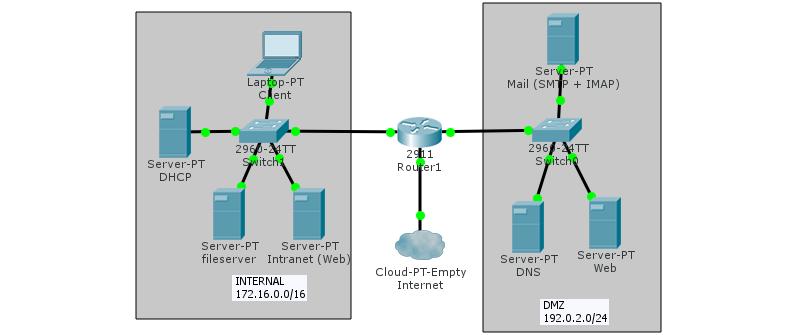
\includegraphics[width=\textwidth]{img/assignment-sme.png}
  \caption[Netwerkdiagram SME-opdracht]{Diagram van het op te zetten kantoornetwerk in de SME-opdracht. Links van de router bevindt zich het netwerk met publiek toegankelijke services (IP range 192.0.2.0/24), rechts het interne netwerk (172.16.0.0/16) met werkstations en netwerkservices voor intern gebruik. Merk op dat sommige van de vernoemde machines niet tot de opdracht behoren, maar enkel dienen als illustratie.}
  \label{fig:sme}
\end{figure}

Deze opdracht bestaat uit een aantal deeltaken:

\begin{itemize}
\item LAMP webserver
\item DNS server
\item Fileserver
\item DHCP server
\item Integratie, configuratie router
\end{itemize}

\subsection{High availability}
\label{subs:high-availability}

In de tweede opdracht verkennen we de taken van een \textit{site reliability engineer (SRE)}. Het is de bedoeling om de infrastructuur op te zetten voor een grote website die veel webtrafiek moet kunnen verwerken. Typisch worden de netwerkservices die samen de klassieke LAMP-stack vormen verdeeld over verschillende machines (zie Figuur~\ref{fig:ha}):

\begin{itemize}
\item Een \textit{load-balancer} verdeelt netwerktrafiek over \textit{verschillende webservers};
\item Een \textit{cache-systeem} zorgt dat niet alle requests leiden tot het opnieuw genereren van een pagina;
\item De \textit{database-backend} komt op een aparte server.
\end{itemize}

Bij dit soort opstellingen is het ook essentieel dat de beheerder een overzicht heeft van de correcte werking van alle componenten. Om dit te realiseren moet je een monitoring-systeem implementeren met een dashboard dat een overzicht geeft van het platform. Je moet in het bijzonder in staat zijn om de \textit{bottleneck resource} te identificeren, de hardware- of systeembron die het eerst verzadigd wordt door de binnenkomende trafiek. Dat kan de CPU zijn, het geheugen, I/O (netwerk of opslag), enz.

\begin{figure}
  \centering
  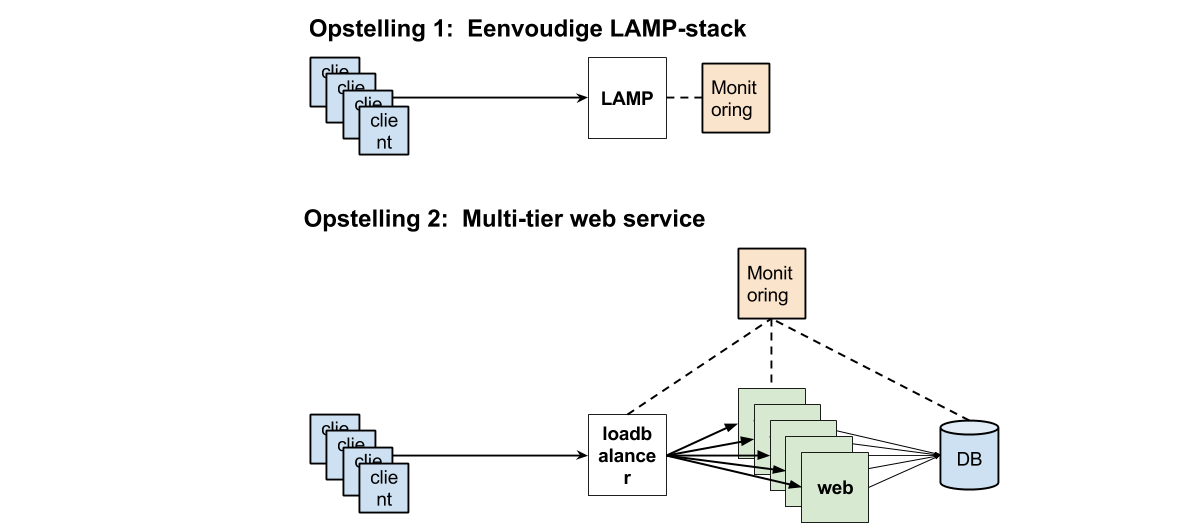
\includegraphics[width=\textwidth]{img/assignment-ha.png}
  \caption[Netwerkdiagram High Availability-opdracht]{Netwerkdiagram High Availability-opdracht. In een eerste opstelling draait de webserver in zijn geheel op een enkele VM met een monitoringsysteem voor de opvolging. Het einddoel is een opstelling waar alle services op aparte entiteiten draaien: een loadbalancer die requests verdeelt over een aantal webservers en een aparte database in de backend.}
  \label{fig:ha}
\end{figure}

\subsection{Continuous Integration/Continuous Delivery}
\label{subs:continuous-delivery}

Het derde jobprofiel dat je kan verkennen is dat van de \textit{release engineer}. Deze komt vooral voor in omgevingen waar webapplicaties de omzet van het bedrijf genereren, zoals bijvoorbeeld grote websites als Google, Amazon, Facebook, enz. De release engineer ondersteunt een team van software-ontwikkelaars om zo snel en zo vlot mogelijk nieuwe features in productie kunnen brengen. In plaats van grote, ingrijpende releases over langere periodes met veel nieuwe features, streeft men er tegenwoordig naar om kleinere releases te doen aan een hoger tempo (soms zelfs tientallen per dag), met bv.~slechts één nieuwe feature of verbetering. Voor deze manier van werken is specifieke infrastructuur nodig en is het nodig een aantal zaken verregaand te automatiseren.

De bedoeling van deze opdracht is om een Continuous Delivery ``build pipeline'' te bouwen voor een zelf te kiezen casus.

Typisch verloopt dat proces volgens deze stappen:

\begin{itemize}
\item De ontwikkelaar werkt op een ``development environment'' in de vorm van een virtuele machine aangestuurd door Vagrant
\item Wanneer de ontwikkelaar code publiceert op de ``master'' branch van een Git repository wordt het buildproces opgestart, bestaande uit:

  \begin{itemize}
  \item code-analyse, linting;
  \item compilatie (indien van toepassing);
  \item uitvoeren van unit tests;
  \item packaging (bv.~RPM, .deb, tarball);
  \item deployment in QA-omgeving (QA: Quality Assurance);
  \item uitvoeren van functionele tests;
  \item deployment in productie-omgeving.
  \end{itemize}

\item De ``QA environment'' is een VM op een zelf te kiezen virtualisatieplatform (bv. KVM, OpenNebula, Docker)
\item Wanneer alle tests slagen, wordt de nieuwe code automatisch gepromoveerd naar de volgende stap, in het beste geval tot en met de ``productie-omgeving'' op een cloud-platform (bv. Amazon AWS of DigitalOcean).
\end{itemize}

Je moet de hele pipeline kunnen demonstreren. Na een wijziging in de code te pushen moet je (na verloop van tijd) de wijziging op de productieserver kunnen zien.

De VMs die op de verschillende platformen draaien, worden toch zo identiek mogelijk geconfigureerd. Hier bestaan tools voor, bv.~Packer.  Je mag ook containers (bv. Docker) gebruiken om je applicatie in te pakken. De build server kan Jenkins zijn, je kan ook kijken naar Travis CI of Gitlab. Voor het laatste kan je gebruik maken van een abonnement op het Gitlab Gold Plan. Indien je hiermee wil werken, neem dan contact op met \href{mailto:bert.vanvreckem@hogent.be}{Bert Van Vreckem}.

Enkele concrete suggesties volgen hieronder. Behalve de Drupal-opdracht zijn dit allemaal reële casussen. Neem contact op met \href{mailto:bert.vanvreckem@hogent.be}{Bert Van Vreckem} indien je interesse hebt in deze opdrachten.

\begin{itemize}
  \item ASP.NET-applicatie op Docker\footnote{\url{https://www.docker.com/}}. Dit is een reële casus en het resultaat is in het beste geval een opstelling die in productie zal gebruikt worden binnen HOGENT. Recentelijk is er een nieuwe applicatie geschreven voor de administratieve opvolging van stages binnen de opleiding toegepaste informatica. Deze draait echter nog niet in productie. Jouw taak zou dan zijn om er voor te zorgen dat de applicatie kan worden gecompileerd en uitgerold in de productie-omgeving. De applicatie is geschreven om in Docker te draaien, dus via deze casus krijg je ook de kans daar ervaring mee op te doen. 
  
  \item Android application development. Dit is een reële casus en bestaat uit het verbeteren en stroomlijnen van een proof-of-concept van een Jenkins build-server voor het compileren van Android applicaties die op Google cloud draait.
  
  \item Geautomatiseerd testen van Ansible-rollen met Molecule\footnote{\url{https://github.com/ansible/molecule}}. Ook dit is een reële casus. De rollen \texttt{bertvv.bind}, \texttt{bertvv.vsftp}, enz. worden getest via Travis CI\footnote{Zie bijvoorbeeld \url{https://travis-ci.org/bertvv/ansible-role-bind}}. Voor elke ondersteunde Linux-distributie wordt een Docker-container opgestart waarop de Ansible-rol toegepast wordt, waarna er acceptatie-tests op uitgevoerd worden. Het testsysteem is ontwikkeld op een moment dat er nog geen algemeen gebruikte oplossingen bestonden voor het doorgedreven testen van Ansible-rollen. Het is gebaseerd op een shell-script en Docker images die specifiek voor deze toepassing zijn opgezet. Het onderhouden van de testinfrastructuur neemt veel tijd in beslag en regelmatig falen de tests omwille van fouten in het testsysteem. Molecule is een relatief nieuw systeem dat recent als het officiële Ansible-testplatform is verkozen. De bedoeling hier is om een proof-of-concept op te zetten voor het testen van de \texttt{bertvv.*}-rollen op basis van Molecule.
  
  \item Automatisch genereren van PDF-bestanden uit \LaTeX{}-broncode en publicatie op Github. De bedoeling is hier om vanuit een Github-repo met \LaTeX-{}be\-stan\-den bij elke push in Travis-CI een build-omgeving op te zetten, het bestand te compileren (incl.~bibliografie, index, enz.), en de resulterende PDF te publiceren op Github, onder Releases. Het systeem moet in staat zijn om bestanden met de HOGENT huisstijlsjablonen te compileren, waarvoor o.a. specifieke fonts nodig zijn (bv. Montserrat). In Travis-CI moet je alle nodige packages downloaden en installeren, wat veel tijd in beslag neemt. Een mogelijke benadering is vooraf een Docker-container te prepareren waar de compilatie in kan uitgevoerd worden\footnote{Bijvoorbeeld \url{https://github.com/Vincevrp/docker-tex}}. Die kan ook lokaal getest worden, wat tijd bespaart bij het troubleshooten.

  \item Ontwikkelen van Drupal plugins. De developer krijgt een VM met Drupal die toelaat om code te schrijven op het hostsysteem en die onmiddellijk zichtbaar is (bv. via VirtualBox shared Folders). Bij committen van code in het versiebeheersysteem worden linters/code analyzers uitgevoerd en geautomatiseerde tests. Eventueel kunnen tests op verschillende versies van PHP/MySQL/Drupal in parallel uitgevoerd worden. Als dit lukt, wordt een package gecreëerd dat kan gepubliceerd worden voor gebruikers.
\end{itemize}

\textbf{Opmerking.} Studenten die deze opdracht combineren met het DevOps-project wordt gevraagd om voor dit vak een andere casus te kiezen. Hetzelfde werk indienen voor twee verschillende vakken is een oneerlijk voordeel dat andere studenten niet hebben. Je kan wel voor beide vakken dezelfde achterliggende technologieën gebruiken zodat je de opgedane kennis wel in beide kan toepassen.

\section{Actualiteit}
\label{sec:actualiteit}

Bij elke rol in de ict-sector is het voortdurend bijwerken van je vakkennis onontbeerlijk om de snelle evolutie in je vakgebied bij te kunnen benen. In Linux systeembeheer is dat niet anders. Wat ons vakgebied kenmerkt is een uitgesproken wil om informatie en kennis te delen. \emph{Sharing is caring!} Er is dan ook een schat van informatie te vinden over de meest recente evoluties via blogs, conferenties waarvan de lezingen op Youtube of Vimeo gepubliceerd zijn, enz.

De bedoeling van deze taak is aan te tonen dat je deze evoluties ook opvolgt en probeert toe te passen in de praktijk. Je kan kiezen uit twee manieren om dit aan te tonen:

\begin{itemize}
  \item Pas een recentelijk gepubliceerde techniek, tool, \ldots{} toe op de opstelling van je hoofdopdracht;
  \item Doe een bijdrage aan een open source project gerelateerd aan de cursus (incl. tools en projecten die door de lector onderhouden worden\footnote{\url{https://github.com/bertvv/}}).
\end{itemize}

Samenwerken met één of enkele medestudenten is toegelaten. In dat geval moet elke student individueel kunnen aantonen een significante bijdrage geleverd te hebben via duidelijke rapportering, Git commits, \ldots

\textbf{Begin zo snel mogelijk hier aan te werken!} Wacht niet tot het einde van het semester om dan snel iets in elkaar te flansen. Dit kan leiden tot een beoordeling ``nog niet bekwaam,'' met als gevolg dat je niet kan slagen.

\subsection{Nieuwe technieken uitproberen}
\label{subs:nieuwe-technieken-uitproberen}

Zoals eerder aangegeven, vormen Linux-systeembeheerders een ``community'' waar er veel informatie uitgewisseld wordt. Sommigen gieten zaken die ze bijleren in een blog-artikel, gaan erover spreken op conferenties, enz.

De bedoeling hier is om zo'n artikel of lezing toe te passen op de labo-opdracht. Een paar voorbeelden als inspiratie:

\begin{itemize}
  \item \textcite{Hayden2015} en \textcite{Davila2015} beschrijven een manier om RHEL of CentOS-sys\-te\-men te testen op vlak van beveiliging, gebaseerd op Ansible. Is het mogelijk dat toe te passen op onze systemen? In het artikel gaat het over versie 6, terwijl wij op versie 7 zitten. In hoeverre kan dit aangepast worden?
  \item Gerelateerd aan het vorige voorstel: voer een security-audit uit met Lynis\footnote{\url{https://cisofy.com/lynis/}} op de VMs in je opstelling. Tracht de belangrijkste problemen op te lossen en verwerk dit in de Ansible-rollen die je gebruikt hebt. Dien eventueel een Pull Request in bij het Github-project van die rol.
  \item Fail2ban is een Intrusion Prevention System dat een server kan beschermen tegen brute-force of denial of service-aanvallen \autocite{Sawiyati2014}. Kan je dit toepassen op onze servers? Het is uiteraard wel de bedoeling dit via Ansible te doen. Dat kan hetzij via een bestaande rol (zie Ansible Galaxy), die je zo nodig aanpast, hetzij één die je zelf schrijft.
  \item Secure Shell is de standaard manier om Linux-servers op een veilige manier van over het netwerk te beheren. Maar volgens \textcite{stribika2015} is het mogelijk om \texttt{sshd} nog beter te beveiligen. Kan je dit toepassen op onze servers? Kan je eventueel een Ansible-rol voor het beher van \texttt{sshd} gebruiken en verbeteren op basis van het artikel?
  \item Zoals onze opstelling nu is, zullen wachtwoorden in de \texttt{host\_vars} of \texttt{group\_vars} bestanden opgeslagen worden. Dit is niet ideaal: we steken onze code in een versiebeheersysteem, maar wachtwoorden horen daar met het oog op beveiliging helemaal niet in thuis. Ansible heeft hiervoor een oplossing: Ansible Vault\footnote{\url{https://docs.ansible.com/ansible/playbooks_vault.html}}. \textcite{Blanc2015} beschrijft een methode om het gebruik van Ansible Vault zo transparant mogelijk te maken. Kan je het toepassen in onze opstelling?
  \item \textcite{Johnson2015} schreef een artikel over het versnellen van Ansible. Kloppen zijn aanbevelingen? Kan je dat aantonen, m.a.w. het tijdverschil meten tussen de standaardinstellingen en zijn aanpassingen?
\end{itemize}

Je kan de blogs waar naar gerefereerd werd in deze voorbeelden opvolgen (bv. via een RSS reader), hieronder volgen er nog enkele:

\begin{itemize}
\item AT Blog: \url{http://www.atcomputing.nl/blog/}
\item Cron Weekly newsletter: \url{https://www.cronweekly.com/}
\item Erika Heidi: \url{http://erikaheidi.com/blog/}
\item Everything Sysadmin (Tom Limoncelli): \url{http://everythingsysadmin.com/}
\item Everything is a Freaking DNS Problem (Kris Buytaert): \url{http://www.krisbuytaert.be/blog/}
\item Fedora Magazine: \url{http://fedoramagazine.org/}
\item Linux Action News: \url{https://linuxactionnews.com/}
\item Linux Journal: \url{http://www.linuxjournal.com/}
\item Major.io (Major Hayden): \url{https://major.io/}
\item ma.ttias.be (Mattias Geniar): \url{https://ma.ttias.be/}
\item Planet CentOS: \url{http://planet.centos.org/}
\item Runaway Sequence (Aaron Hunter): \url{http://sharknet.us/}
\item Standalone Sysadmin (Matt Simmons): \url{https://www.standalone-sysadmin.com/blog/}
\item SysadminCasts (Justin Weissig): \url{https://sysadmincasts.com/}
\item The Geek Stuff: \url{http://www.thegeekstuff.com/}
\end{itemize}

Vond je andere interessante blogs? Geef maar door aan de lectoren! Andere bronnen van informatie zijn Youtube of Vimeo (voor presentaties van conferenties of screencasts), Twitter, enz.

Ben je zelf buiten de opleiding om bezig met Linux? Bespreek met de lector of je je ervaringen, experimenten, \ldots{} eventueel kan inbrengen voor deze opdracht.

\subsection{Bijdrage aan een open source project}
\label{subs:bijdrage-aan-een-open-source-project}

Alle tools waar we in de cursus gebruiken zijn open source. Sommige, zoals Ansible, werden door een softwarebedrijf ontwikkeld die daar een businessmodel rond gebouwd hebben. Andere werden door enthousiastelingen in hun vrije tijd ontwikkeld. In elk geval kunnen we gratis gebruik maken van software van hoge kwaliteit, dankzij de inspanningen van velen.

Het is passend daar iets voor terug te doen, dus de bedoeling is om een significante bijdrage te leveren aan een open source project dat gerelateerd is aan de cursus. Dit kan een kleine bijdrage zijn, maar voorwaarde is wel dat ze aanvaard is door de auteur(s) van het project.

Je mag hiervoor samenwerken met één of meerdere medestudenten, maar de individuele bijdrage van elk teamlid moet aantoonbaar zijn (bv. aan de hand van Git commits). Zet hiervoor een aparte, publieke Github repository op, en verwijs er naar vanuit je laboverslag voor deze opdracht.

Enkele mogelijkheden:

\begin{itemize}
  \item Op Ansible Galaxy zijn veel rollen te vinden die beter kunnen, of waar de auteur niet genoeg tijd heeft om zaken toe te voegen of fouten op te lossen. Implementeer een nieuwe feature, zorg er voor dat ze op CentOS 7 draaien, verbeter fouten, \ldots{} Ook de lector apprecieert hulp bij het verder ontwikkelen van zijn Ansible-rollen \url{https://galaxy.ansible.com/bertvv/} en \url{https://github.com/search?q=user\%3Abertvv+ansible}.

  Het resultaat wordt ingediend als een Pull Request, de code volgt de richtlijnen voor stijl\footnote{\url{https://github.com/bertvv/ansible-role-skeleton/wiki}}, en wordt getest. Opties zijn niet \emph{hard-coded} maar blijven instelbaar via rolvariabelen. Waar mogelijk wordt een standaardwaarde gekozen die in de meeste gevallen het beste resultaat geeft, of wordt aan de hand van de eigenschappen van het systeem een waarde ``berekend'' of bepaald die voor dat systeem optimaal is. Alle nieuwe variabelen/features worden goed gedocumenteerd.
  
  Voor concrete ideeën kan je de Issues bekijken op het Github-project en één ervan op je te nemen.

  \item Schrijf een Ansible rol (waar nog geen alternatief voor CentOS voor bestaat) en publiceer die op Ansible Galaxy. Dit doe je best in samenwerking met één of meerdere medestudent(en)! Wanneer je voor de hoofdopdracht een nieuwe Ansible rol schrijft, kan je die algemeen bruikbaar maken en publiceren.
  
  \item Pas een techniek die beschreven is voor een andere distributie (CentOS 6, Debian, Ubuntu, \ldots{}) toe op CentOS 7. In de vorige sectie vind je een paar concrete voorbeelden.
\end{itemize}

Andere ideeën zijn ook welkom, bespreek die met de lector. Ook op Chamilo kan je nog enkele voorstellen vinden.

\section{Rapportering en documentatie}
\label{sec:rapportering-en-documentatie}

In de \texttt{assignment/} directory van je repository komt alle documentatie terecht in verband met de labo-taken. Het gebruikte formaat is Markdown~\autocite{Gruber2004,Github2016}, wat de standaard geworden is voor documentatie op Github (en ook andere Git hosting-oplossingen zoals Gitlab of Bitbucket). Markdown is een eenvoudig tekstformaat dat kan gerenderd worden als HTML, of makkelijk naar andere formaten kan omgezet worden (PDF, \LaTeX\, presentatie met reveal.js, enz.). Leer het formaat goed kennen en controleer of je verslagen duidelijk leesbaar zijn (op Github of reeds lokaal met een editor met Markdown-ondersteuning). Gebruik bv. codeblokken met syntax colouring, links naar relevante code elders in de repository, enz.

\subsection{Laboverslagen}
\label{subs:laboverslagen}

Er is een sjabloon voorzien voor de laboverslagen. Pas dit sjabloon aan voor jezelf, vul bovenaan je naam in. Voor elke deeltaak maak je een apart verslag, waar je in detail uitlegt wat je precies gedaan hebt. Hoe heb je de taak aangepakt? Welke bronnen heb je gebruikt? Reflecteer ook over je vooruitgang: wat ging goed/niet goed? Wat heb je geleerd? Waar zit je vast, waar heb je nog problemen mee? Let wel: het is niet de bedoeling om code te gaan knippen en plakken in je laboverslag!

Bij elk laboverslag hoort een testplan en -rapport. Het testplan is een opsomming van alle handelingen die nodig zijn om aan te tonen dat het op te zetten systeem zich gedraagt volgens de specificaties.

Het testplan is eigenlijk het scenario van de demo die je geeft aan de lector om aan te tonen dat je alle aspecten van de opdracht correct hebt uitgevoerd. Dit bestaat uit concrete handelingen of commando's die je moet uitvoeren, en een beschrijving van het verwachte resultaat.

Door het lezen van het testrapport moet het duidelijk zijn in hoeverre de opdracht is uitgevoerd, wat het effectieve resultaat van de tests was. Je kan transcripties toevoegen van de terminal (gebruik hiervoor Markdown codeblokken, geen screenshots!). Het testrapport zou evenveel informatie moeten bevatten als de demo.

Ook bij de \textbf{troubleshooting-oefeningen} hoort een verslag. Deel je verslag op in secties voor de verschillende fasen in het troubleshooting-proces. Je kan je verslag al voorbereiden door de commando's die je zeker moet uitvoeren er alvast in op te sommen, samen met verwachte resultaten (voor zover dit al op voorhand kan). Sla dit op als een apart sjabloon specifiek voor troubleshooting. Bij het uitvoeren van de oefening kan je dit dan aanvullen met de effectieve resultaten die je krijgt, en de commando's/configuratiewijzigingen die je hebt uitgevoerd om problemen op te lossen.

\subsection{Cheat-sheets en checklists}
\label{subs:cheat-sheets-en-checklists}

Wanneer je niet gewend bent om met Linux te werken, dan is het niet evident om op te zoeken en te onthouden welke commando's je nodig hebt voor welke taak. Via Google vind je wel vaak een oplossing, maar dat ligt niet altijd voor de hand. Er zijn bijvoorbeeld recentelijk substantiële wijzigingen doorgevoerd in de architectuur van de belangrijkste Linux-distributies waardoor bepaalde commando's (die je erg vaak tegenkomt bij Googlen) niet meer werken.

Om jezelf te helpen bij het onthouden van de belangrijkste commando's, is het bijhouden van een cheat-sheet of ``spiekbriefje'' een nuttig hulpmiddel. Als je een bepaald commando een paar keer bent moeten gaan opzoeken, dan is het best dat eens te noteren zodat je het in de toekomst sneller terugvindt en op de duur ook beter onthoudt.

Hetzelfde geldt voor procedures van handelingen die steeds terugkomen.  Bijvoorbeeld, als je wil nagaan of de IP-instellingen van een host kloppen, gebruik je altijd dezelfde commando's. Wanneer je die telkens opnieuw moet gaan opzoeken verspil je tijd en het is best mogelijk dat je zo zaken over het hoofd ziet. Door checklists bij te houden, verminder je het opzoekwerk en kan je ook vlotter werken~\autocite{Simmons2009}.

Je kan inspiratie opdoen op deze Github-repository waar een aantal cheat-sheets en checklists gepubliceerd zijn: \url{https://github.com/bertvv/cheat-sheets}.

Bij de evaluatie wordt er rekening mee gehouden hoe je deze documenten hebt bijgehouden in de loop van het jaar (aan de hand van de commit log).

\subsection{Bloggen}
\label{subs:bloggen}

Technische blogs zoals deze die eerder aangehaald werden zijn een meer en meer voorkomende manier om ervaringen en informatie uit te wisselen binnen ons vakgebied. Studenten die gaan solliciteren (en ook wie al in het vak staat) kunnen met een eigen blog aan potentiële werkgevers aantonen dat ze gepassioneerd zijn door hun vak, bezig zijn met de laatste technologieën en open staan voor het delen van kennis. Je kan een eigen blog opstarten en schrijven over wat je in deze cursus (en ook andere!) leert, zaken die je zelf opgezocht en ondervonden hebt, \ldots

Voorbeeldjes:

\begin{itemize}
\item Jürgen Van Meerhaeghe: \url{https://jurgenvm.blogspot.be/}
\item Stijn Spanhove: \url{http://www.spanhove.com/blog.htm}
\item Thomas Clauwaert: \url{https://ciberth.blogspot.be/}
\item Toon Lamberigts en Tomas Vercautter: \url{https://t0t0.github.io/}
\end{itemize}

Dit is vrijblijvend, maar heeft wel een positieve invloed op je examencijfer.


\chapter{Aan de slag}
\label{ch:aan-de-slag}

In dit hoofdstuk vind je wat technische achtergrond over een aantal onderwerpen die in de labo-opdrachten aan bod kunnen komen. Alles wat hier meegegeven wordt is gebaseerd op jarenlange ervaring, en typische problemen die studenten tegenkomen.

De bedoeling is om een minimum aan informatie mee te geven om je in staat te stellen snel aan de slag te gaan en een aantal typische beginnersfouten te vermijden. Voordat je aan de opdracht begint, lees je dus best eerst de informatie hier na en ga je ook best de \textbf{gerefereerde bronnen opzoeken en bestuderen}!

\section{Opzetten werkomgeving}
\label{sec:opzetten_werkomgeving}

Installeer eerst de nodige software, meer bepaald de laatste stabiele versie van de applicaties opgesomd in Sectie~\ref{ssec:software}. De volledige neerslag van al wat je voor deze cursus doet wordt bijgehouden in het versiebeheersysteem Git. Via Chamilo vind je een link die, als je er op doorklikt, een nieuwe repository creëert waar je in kan werken. Deze is zichtbaar voor jou en de lector. Naast de configuratie van de opgezette systemen zal je er ook je documentatie bijhouden, zoals testrapporten, procedures, cheat sheets en checklists.

Richtlijnen voor het opstarten van je Git project:

\begin{enumerate}
  \item In principe moet je al een Github account hebben. Als je dit nog niet gedaan hebt, koppel dan zeker je @student.hogent.be adres aan het account. Je kan dan het Github Student Developer Pack\footnote{\url{https://education.github.com/pack}} aanvragen met allerlei interessante aanbiedingen.
  \item Maak een SSH-sleutelpaar aan om het pushen naar Github te vereenvoudigen. Het commando is \texttt{ssh-keygen}, volg de richtlijnen die het geeft. Geef voor je gemak een lege \emph{passphrase} op (zoniet moet je telkens je de sleutel gebruikt je passphrase intikken). Normaal zou er in de directory \path{~/.ssh}\footnote{Het symbool {\textasciitilde} is natuurlijk de \emph{home directory} van de gebruiker. In Linux komt dit overeen met \path{/home/USER}, onder Windows met \path{C:\Users\USER} of \path{C:\Gebruikers\USER}, onder MacOS met \path{/Users/USER}} twee bestanden aangemaakt moeten zijn: \path{id_rsa} en \path{id_rsa.pub}. Het eerste is je private sleutel (die je geheim moet houden), het tweede de publieke. Die laatste kan je op Github registreren via je profielinstellingen (klik op je avatar rechtsboven, volg \emph{Settings} en dan \emph{SSH and GPG keys}).

  \item Basisconfiguratie Git, indien je dit nog niet gedaan hebt (kijk na in het configuratiebestand \path{~/.gitconfig}):

    \begin{minted}[gobble=6]{console}
      $ git config --global user.name "VOORNAAM NAAM"
      $ git config --global user.email "VOORNAAM.NAAM@student.hogent.be"
      $ git config --global push.default simple
      $ git config --global core.autocrlf input
      $ git config --global pull.rebase true
    \end{minted}

  \item Maak lokaal een directory aan die je voorbehoudt voor al wat met deze cursus te maken heeft. Binnen deze directory kan je je Github-repository klonen. Klik op de Github-pagina van je repository op de groene knop rechts (\emph{Clone or download}), kies voor ``Clone with SSH'' kopieer de link van de vorm \path{git@github.com:HoGentTIN/REPO_NAAM-GEBRUIKERSNAAM.git}.

    \begin{minted}[gobble=6]{console}
      $ cd Documents/Courses/EnterpriseLinux/
      $ git clone git@github.com:HoGentTIN/REPONAAM-GEBRUIKERSNAAM.git repo
    \end{minted}

  Dit maakt een lokale kopie van de repository in een subdirectory \path{repo}. Je kan zelf de naam van deze directory kiezen en die achteraf verplaatsen, alles blijft gewoon werken.
  
  \item Creëer een nieuwe \emph{branch} met de naam \texttt{solution} om je eigen code en documentatie bij te houden. Verderop wordt duidelijk waarom dit belangrijk is.

    \begin{minted}[gobble=6,linenos=false]{console}
      $ git checkout -b solution
    \end{minted}

  \item Bekijk de bestanden in de \path{assignment/} directory. Hier vind je de opgave van deelopdrachten en sjablonen voor verslagen en cheat sheets in Markdown-formaat~\autocite{Gruber2004}. Pas alvast het sjabloon aan, vul er je eigen naam in.
\end{enumerate}

Wanneer er errata in de opgave gepubliceerd worden, kan je die relatief eenvoudig binnen halen, maar enkel als je een eigen branch aangemaakt hebt.

\begin{enumerate}
  \item Eerst moet je zorgen dat je updates kan binnenhalen van de repository met de opdracht. Het volgende commando zorgt dat je kan synchroniseren met die repository. Dit moet slechts één keer gebeuren.

    \begin{minted}[gobble=6,linenos=false]{console}
      $ git remote add upstream https://github.com/HoGentTIN/elnx-sme.git
    \end{minted}

  \item Wanneer er nieuwe commits gebeurd zijn in de opgave, kan je de wijzigingen telkens zo ophalen:

    \begin{minted}[gobble=6]{console}
      $ git checkout master
      $ git pull upstream master
      $ git checkout solution
      $ git rebase master
    \end{minted}

    \begin{itemize}
      \item De eerste twee regels zorgen er voor dat jouw versie van de master-branch up-to-date gebracht wordt met de nieuwe commits.
      \item In de derde regel ga je opnieuw naar je eigen branch. Voorlopig is er daar nog niets gewijzigd
      \item In de vierde regel, tenslotte, ga je de wijzigingen in de opgave op jouw eigen versie toepassen. Mogelijks komen er hier conflicten naar boven tussen bepaalde bestanden in de opgave en jouw wijzigingen. Lees goed de instructies die Git hier geeft om deze conflicten op te lossen.
    \end{itemize}

Deze procedure werkt niet als je geen branch voor je eigen oplossing gemaakt hebt. In dat geval haal je jezelf een hoop ellende op de hals\ldots

\end{enumerate}

\section{Algemene richtlijnen}
\label{sec:algemene_richtlijnen}

In deze sectie vind je enkele algemene richtlijnen die je helpen vlotter en efficiënter te werken.

\begin{itemize}
  \item Voor je aan een (deel-)opdracht begint, bereid je eerst voor door alle aangereikte studiematerialen te bestuderen: handleidingen, screencasts, \ldots Die ``van buiten blokken'' is helemaal niet nodig, maar zorg er in elk geval voor dat je er in die mate vertrouwd bent, dat je snel gericht kan zoeken naar juiste, relevante informatie. Je vindt die via de bronvermeldingen in deze syllabus, of via de opgave
  \item Open \textbf{verschillende terminalvensters/consoles naast elkaar} (zie Figuur~\ref{fig:screenshot-terminals}). Elke terminal krijgt zijn eigen functie, bijvoorbeeld:
    \begin{itemize}
      \item Vim editor (of VS Code/Sublime/Notepad/\ldots in een apart venster);
      \item doorvoeren van wijzigingen aan de configuratie;
      \item ingelogd op VM, voor commando's;
      \item ingelogd op VM, voor tonen logbestanden.
    \end{itemize}
  \item \textbf{Werk stap voor stap.} Schrijf niet teveel code ineens. Probeer eerst een minimaal werkende opstelling te verkrijgen en registreer meteen in Git. Maak minimale wijzigingen en \textbf{test elke wijziging uit}. Hoe groter en ingrijpender de wijzigingen, hoe meer kans op fouten en hoe moeilijker die te debuggen zijn. Zodra iets werkt, en je bent een stap verder, registreer je dit meteen in Git en geef je een duidelijke, beschrijvende commit-boodschap.
  \item \textbf{gebruik Git op de command-line.} Bij de meeste Git commando's krijg je gedetailleerde uitleg over hoe je een stap verder moet gaan en ook hoe je de laatste stap kan ongedaan maken. Dit geeft op de duur een beter inzicht in hoe Git precies werkt.
  \item Probeer \textbf{elke commit te beperken tot één enkele ``reden''} om wijzigingen aan te brengen aan de bestaande code. Dit maakt de ``geschiedenis'' van je project transparanter en maakt ook dat je makkelijker kan terugkeren naar een bepaalde stap wanneer je de mist in gaat.
  \item \textbf{Maak backups} van de originele, ongewijzigde configuratiebestanden zodat je er op kan terugvallen als er iets misloopt. Soms heb je zodanig zitten ``prutsen'' dat je er niet meer in slaagt de service te laten werken.
  \item \textbf{Gebruik \texttt{vagrant destroy}} (zie Sectie~\ref{sec:vagrant}). Wanneer je veel manuele wijzigingen hebt aangebracht in een VM, ben je op de duur niet meer zeker dat die zich in de gewenste toestand bevindt. Of je kan door experimenteren de VM onbruikbaar gemaakt hebben. Door de VM te verwijderen en opnieuw op te bouwen (met \texttt{vagrant up}) kan je opnieuw beginnen van een werkende versie (als je de vorige richtlijnen opvolgt, tenminste!).
  \item Ook wanneer je denkt klaar te zijn met een deelopdracht, genereer de VM nog eens helemaal opnieuw en voer alle acceptatietests uit.
\end{itemize}

\begin{figure}
  \centering
  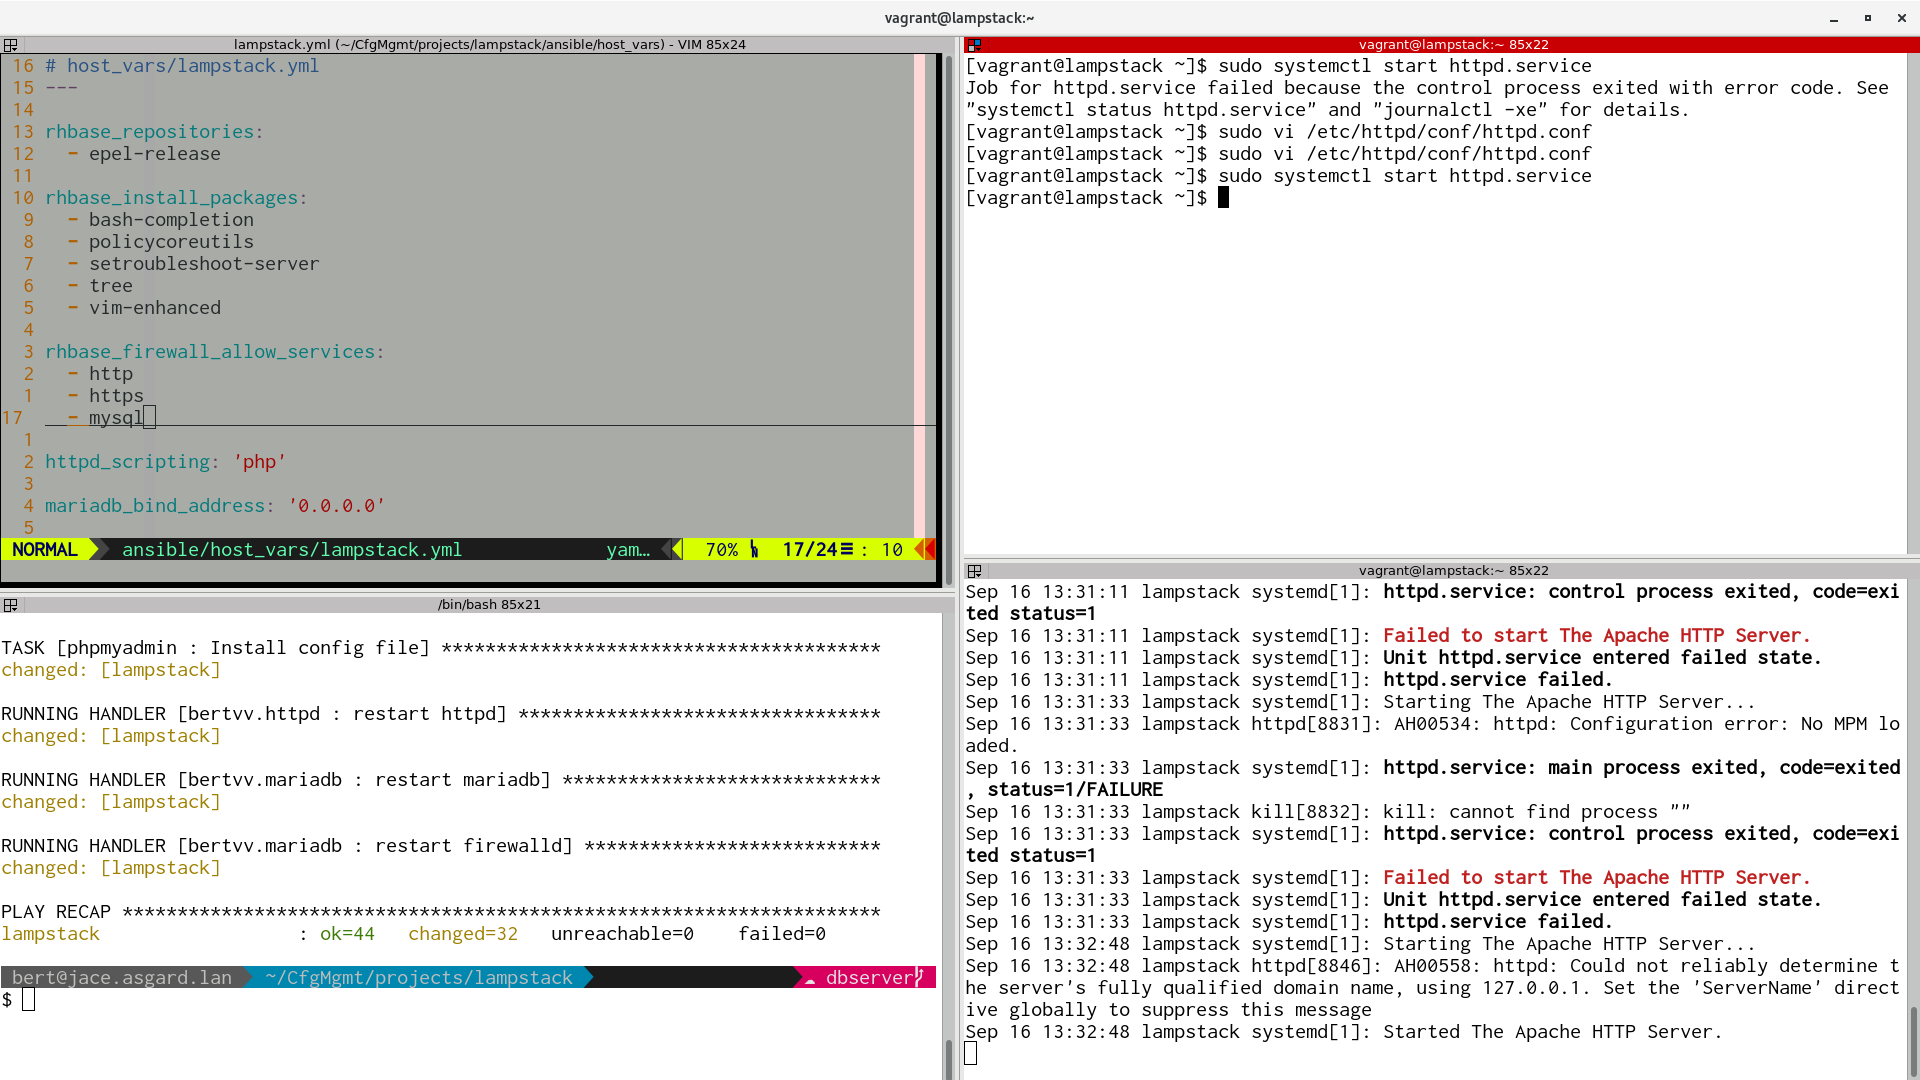
\includegraphics[width=\linewidth]{img/screenshot-terminals}
  \caption[Gebruik van verschillende terminals.]{\textbf{Gebruik van verschillende terminals.} In deze schermafbeelding is Terminator (een terminal-applicatie voor Linux) opgedeeld in vier aparte shells. Linksboven is Vim geopend met een broncodebestand. De terminal linksonder wordt gebruikt om wijzigingen in de broncode door te voeren op de virtuele machines. Rechtsboven is er ingelogd op de virtuele machine waar momenteel wijzigingen op aangebracht worden en kunnen commando's uitgevoerd worden om zaken uit te proberen of problemen op te sporen. Rechtsonder, tenslotte, worden relevante logbestanden van de VM getoond.}
  \label{fig:screenshot-terminals}
\end{figure}

\section{Bash tips}
\label{sec:bash_tips}

In deze sectie vind je een aantal tips voor het gebruik van de Bash-shell. In deze cursus maak je intensief gebruik van de shell, en het loont de moeite om Bash wat beter te leren kennen. Het zit immers vol met interessante features die je toelaten productiever te werken. Online is hier nog veel meer over te vinden~\autocite{Rowe2009}.

De tips hier gelden ook voor Windows- en MacOS-gebruikers! Windows-gebruikers hebben beschikking over een recente versie van Bash via Git (Git Bash). In MacOS X zit ook een Bash-shell, weliswaar een zeer oude versie\footnote{Dit is omwille van de softwarelicentie. Recente versies van Bash vallen onder de open source GPL-licentie, waar Apple niets mee te maken wil hebben.}. Je kan een recente versie installeren via HomeBrew\footnote{\url{http://brew.sh}}.

\begin{itemize}
  \item \textbf{Gebruik \emph{\texttt{TAB}-completion}.} Je kan een deel van een commando of pad intikken en dan de \texttt{TAB}-toets indrukken. Indien mogelijk zal Bash het woord vervolledigen, of mogelijke alternatieven tonen. Als je de package \texttt{bash-completion} installeert zijn er nog veel meer mogelijkheden.
  \item \textbf{Gebruik de \emph{command history}.} Bash houdt de commando's die je eerder gebruikt hebt bij. Met de pijltjestoetsen kan je eerdere commando's terug halen. Gebruik \texttt{Ctrl-R} om te zoeken in de command history. Je kan dan een fragment van het commando intikken, Bash toont dan het laatste commando waar dat tekstfragment in voorkomt.
  \item \textbf{Bang bang!} In Bash zijn er enkele shortcuts voorzien voor (delen van) het vorige commando. \texttt{!!} staat voor het gehele vorige commando, \texttt{!\$} voor het laatste argument en \texttt{!*} voor alle argumenten. Een voorbeeldje van het gebruik:

    \begin{minted}{console}
$ yum update
You need to be root to perform this command.
$ sudo !!
sudo yum update
[...]
$ mkdir -p some/long/path/i/dont/want/to/repeat
$ cd !$
cd some/long/path/i/dont/want/to/repeat
$
\end{minted}
  \item \textbf{Toetsenbordcombinaties.} Naast \texttt{Ctrl-R} van hierboven zijn er nog een aantal nuttige toetsenbordcombinaties.
    \begin{itemize}
      \item \texttt{Ctrl-C} onderbreekt het huidige proces
      \item \texttt{Ctrl-Z} pauzeert het huidige proces (haal het terug met \texttt{fg})
      \item \texttt{Ctrl-D} sluit de shell af (enkel op lege regel)
      \item \texttt{Ctrl-K} verwijdert de tekst rechts van de cursor
      \item \texttt{Ctrl-U} verwijdert de tekst links van de cursor
      \item \texttt{Ctrl-T} verwisselt letterteken onder de cursor met dat voor de cursor
      \item \texttt{Alt-T} verwisselt woord voor met woord na de cursor
    \end{itemize}

    Er bestaan nog \emph{veel} meer combinaties. Deze kan je vinden in de man-pagina \texttt{bash(1)} in de sectie READLINE (subsectie \emph{Readline Command Names} en volgende).

  \item \textbf{Personaliseer de shell.} Je kan het gedrag van de shell in hoge mate aan je eigen wensen aanpassen door het bestand \path{~/.bashrc} aan te passen. Je kan het gedrag van tab-completion of de command history aanpassen, een eigen commandoprompt instellen, aliassen (zie verder) of functies definiëren, enz. Het zou ons te ver leiden om alle mogelijkheden uit te diepen, maar je kan een relatief eenvoudig voorbeeld vinden in \url{https://github.com/bertvv/server-dotfiles/} (installatie-instructies te vinden in de README), en een meer uitgebreid voorbeeld in \url{https://github.com/bertvv/dotfiles/} (of gelijknamige repositories van andere Github-gebruikers).

  \item \textbf{Aliassen} zijn een soort shortcuts voor commando's die je vaak gebruikt. Dit kan enorm veel typwerk besparen. Je kan ze toevoegen in je \path{~/.bashrc}. Enkele voorbeelden ter inspiratie:

    \begin{minted}{bash}
alias l='ls -l --si --time-style=long-iso --color'
alias a='git add'
alias c='git commit -m'
alias h='git log --pretty="format:%C(yellow)%h %C(blue)%ad %C(reset)%sC(red)%d %C(green)%an%C(reset), %C(cyan)%ar" --date=short --graph --all'
alias s='git status'
alias vu='vagrant up'
alias vD='vagrant destroy'
alias elnx='cd /home/bert/Documents/Courses/EnterpriseLinux/16-17'
\end{minted}

    Nog meer voorbeelden vind je in \url{https://github.com/bertvv/dotfiles/blob/master/.bash.d/aliases.sh}.
\end{itemize}

\section{Vagrant}
\label{sec:vagrant}

Vagrant is een command line tool die het aanmaken en configureren van virtuele machines automatiseert. Het ondersteunt een aantal virtualisatieplatforms, o.a.~VirtualBox, Hyper-V, libvirt, enz. Wij zullen het gebruiken in combinatie met VirtualBox. Voor een demo van de werking van Vagrant, bekijk eerst de screencast van \textcite{Weissig2014}.

Je Git repository bevat een Vagrant-omgeving voor het opzetten van de VMs voor je labo-opdracht. Er zijn alvast twee VMs gedefinieerd.  Je kan een overzicht van de VMs opvragen met (voorbeeld uit de SME-opdracht van Sectie~\ref{subs:smallmedium-enterprise-infrastructure}):

\begin{minted}{console}
$ vagrant status
Current machine states:

router                    not created (virtualbox)
pu001                     not created (virtualbox)

The environment has not yet been created. Run `vagrant up` to
create the environment. If a machine is not created, only the
default provider will be shown. So if a provider is not listed,
then the machine is not created for that environment.
$
\end{minted}

De initiële setup bevat twee virtuele machines met namen \texttt{router} en \texttt{pu001}, respectievelijk. We beginnen met \texttt{pu001}, de router wordt later geconfigureerd.

Start de VM met \texttt{vagrant\ up\ pu001}. De eerste keer dat je dit doet wordt er een basis-VM gedownload met een minimale installatie van de laatste stabiele versie van CentOS. Doe dit best op een performant netwerk: het bekabelde netwerk op de campus of thuis/op kot. Deze ``base box'' wordt bijgehouden en zal telkens dienst doen als basis voor het opzetten van alle hosts in ons netwerk. Het downloaden gebeurt dus slechts één keer-.

Na opstarten kan je inloggen met \texttt{vagrant\ ssh\ pu001}. Je bent ingelogd als gebruiker \texttt{vagrant} en kan commando's uitvoeren met \texttt{root}-rechten door er \texttt{sudo} voor te plaatsen (geen wachtwoord vereist). Als het nodig mocht zijn: het wachtwoord van de gebruikers \texttt{vagrant} en \texttt{root} is telkens \texttt{vagrant}.

Als je \texttt{ls\ /} uitvoert, zal je merken dat er een directory \path{/vagrant} bestaat. Dit is je lokale repository die gemount is binnen de VM. Dit is een eenvoudige manier om bestanden te delen tussen VM en host-systeem.

Let er op dat je VMs niet meer vanuit je VirtualBox GUI opstart of bewerkt. Doe dit nu enkel met Vagrant en vanuit een terminal. Het commando \texttt{vagrant} moet altijd uitgevoerd worden vanuit de directory waar het bestand \texttt{Vagrantfile} zich bevindt.

De belangrijkste Vagrant commando's worden opgesomd in Tabel~\ref{tab:vagrant-commandos}. Daar waar \texttt{[VM]} tussen rechte haken staat, is dat een optioneel argument. Als je het weglaat, wordt de actie op \emph{alle} VMs tegelijk uitgevoerd.

\begin{longtable}{@{}ll@{}}
  \toprule
  Commando & Functie\tabularnewline
  \midrule
  \endhead
  \texttt{vagrant\ status} & Geef een overzicht van de Vagrant-omgeving\tabularnewline
  \texttt{vagrant\ up\ [VM]} & Start \texttt{VM} op\tabularnewline
  \texttt{vagrant\ provision\ [VM]} & Draai het configuratiescript op \texttt{VM}\tabularnewline
  \texttt{vagrant\ ssh\ VM} & Log in op \texttt{VM} als gebruiker \texttt{vagrant}\tabularnewline
  \texttt{vagrant\ halt\ [VM]} & Stop \texttt{VM}\tabularnewline
  \texttt{vagrant\ reload\ [VM]} & Herstart \texttt{VM}\tabularnewline
  \texttt{vagrant\ destroy\ [VM]} & Vernietig \texttt{VM}\tabularnewline
  \bottomrule
\caption{De belangrijkste \texttt{vagrant}-commando's}
\label{tab:vagrant-commandos}
\end{longtable}

Alle VMs in de opstelling krijgen twee netwerkinterfaces:

\begin{itemize}
  \item Adapter 1: NAT-interface (de ``management interface'' voor Vagrant, Internetverbinding voor de VM)
  \item Adapter 2: Host-only interface (gebruikt om vanop het hostsysteem de netwerkservices op de VM aan te spreken)
\end{itemize}

Zorg dat je goed begrijpt hoe deze interfaces werken, zoniet wordt troubleshooten erg moeilijk~\autocite{VanVreckem2015a}.

\section{Ansible}
\label{sec:ansible}

Ansible is een \emph{configuration management system,} d.w.z. het staat in voor het configureren van een host vanaf een minimale installatie tot een volledig operationeel systeem. Het concept van een configuration management tool is dat je beschrijft wat de gewenste toestand van het systeem is, de tool brengt het systeem naar die toestand. Bekijk de screencast van \textcite{Weissig2015} voor een inleiding op Ansible. In een vervolg-screencast wordt ook de combinatie van Ansible en Vagrant belicht. In deze gids geven we enkel wat uitleg om aan de slag te gaan met de startopstelling voor de labo-opdracht, maar als je op zoek bent naar een goed naslagwerk over Ansible, overweeg dan om het e-boek van \textcite{Geerling2016} te kopen. Het boek is al enkele jaren oud, maar de auteur werkt nog verder aan het boek, updates zijn gratis.

Sommige config management systemen hebben een eigen taal ontwikkeld om die configuratie in te beschrijven (bv. Puppet), andere gebruiken een bestaande taal (bv. Chef, configuratie in Ruby). Bij Ansible beschrijf je de configuratie van een systeem met YAML (een variant van JSON), een eenvoudig tekstformaat om data te structureren op een manier die makkelijk te interpreteren is zowel door mensen als computers. De bestanden die deze configuratiecode bevatten worden \emph{playbooks}\footnote{\url{https://docs.ansible.com/ansible/playbooks.html}} genoemd. Als je deze playbooks op een specifieke manier structureert en herbruikbaar maakt, spreekt men van een \emph{rol}\footnote{\url{https://docs.ansible.com/ansible/playbooks_roles.html\#roles}}. Je kan rollen toekennen aan een host, en specifieke instellingen toepassen door het invullen van \emph{variabelen}\footnote{\url{https://docs.ansible.com/ansible/playbooks_variables.html}}. Op Ansible Galaxy\footnote{\url{https://galaxy.ansible.com/}} kan je tientallen rollen vinden die door hun auteurs gepubliceerd zijn.

De directorystructuur van een Ansible-project ligt vast en wordt uitvoerig beschreven in de documentatie\footnote{\url{https://docs.ansible.com/ansible/playbooks_best_practices.html}}.

\subsection{Rollen toekennen aan hosts}
\label{sub:rollen-toekennen-aan-hosts}

Om een rol toe te kennen aan een host, bewerk je de \emph{master playbook} \path{ansible/site.yml}. Dit bestand bevat een overzicht van alle hosts onder het beheer van Ansible, met de rollen van elke host (spaties worden getoond):

\begin{minted}[showspaces]{yaml}
# site.yml
---
- hosts: pu001
  become: true
  roles: []
\end{minted}

Host \texttt{pu001} heeft nog geen rollen toegekend, dat gaan we nu veranderen:

\begin{minted}[showspaces]{yaml}
# site.yml
---
- hosts: pu004
  become: true
  roles:
    - bertvv.rh-base
\end{minted}

Onder \texttt{roles:} kan je zoveel rollen toevoegen als nodig. Let goed op de indentatie. Je \textbf{moet} telkens inspringen met 2 spaties, en alle data op hetzelfde niveau moet links mooi uitgelijnd zijn.

\subsection{Rollen installeren}
\label{sub:rollen-installeren}

Alle rollen die gebruikt worden in \path{site.yml} moeten beschikbaar zijn in de directory \path{ansible/roles/} in een subdirectory met dezelfde naam als deze gebruikt in \path{site.yml}.

De naam van de rol \path{bertvv.rh-base} is geschreven in de vorm \path{AUTEUR.ROLNAAM}. Dit wijst er op dat deze rol op Ansible Galaxy gepubliceerd is. Je kan die daar terugvinden onder de url ``\url{http://galaxy.ansible.com/AUTEUR/ROLNAAM/}.'' Je kan daar de rol downloaden en uitpakken op de juiste plaats in de Ansible-directorystructuur.

Dit is het eenvoudigste als je \textbf{MacOS of Linux} op je hostsysteem draait. Je kan dan Ansible installeren en gebruik maken van het commando \texttt{ansible-galaxy}:

\begin{minted}{console}
$ ansible-galaxy -p ansible/roles install bertvv.httpd
- downloading role 'httpd', owned by bertvv
- downloading role from https://github.com/bertvv/ansible-role-httpd/archive/v1.2.1.tar.gz
- extracting bertvv.httpd to ansible/roles/bertvv.httpd
- bertvv.httpd was installed successfully
$
\end{minted}

Dit commando zal de rol \path{bertvv.rh-base} downloaden en uitpakken onder directory \path{ansible/roles}.

Onder \textbf{Windows} wordt Ansible niet ondersteund, en is dit commando dus ook niet beschikbaar. Je kan wel manueel een rol downloaden van de Github-repository (bijvoorbeeld voor \path{bertvv.rh-base} van \url{https://github.com/bertvv/ansible-role-rh-base/releases}) en dan op de juiste plaats uitpakken.

In je repository is ook een scriptje voorzien dat het installatieproces automatiseert: \path{scripts/role-deps.sh}. Als je het uitvoert in een Bash shell vanuit de hoofddirectory van je repository, zal het in \path{ansible/site.yml} alle rollen die er vernoemd worden van Ansible Galaxy (of indien de rol daar niet gepubliceerd is van Github) downloaden en installeren. Dit script werkt trouwens ook op MacOS en Linux.

\begin{minted}{console}
$ ./scripts/role-deps.sh 
- downloading role 'rh-base', owned by bertvv
- downloading role from https://github.com/bertvv/ansible-role-rh-base/archive/v2.3.0.tar.gz
- extracting bertvv.rh-base to /home/bert/Documents/Vakken/enterprise-linux/opgaven/elnx-sme-bertvv/ansible/roles/bertvv.rh-base
- bertvv.rh-base (v2.3.0) was installed successfully
$ 
\end{minted}

Merk op dat rollen van Ansible Galaxy genegeerd worden door Git. Het heeft geen zin je eigen repository te ``vervuilen'' met code die al elders onderhouden wordt. Het is dus ook de bedoeling dat je \emph{geen wijzigingen} aanbrengt in bestaande rollen. Als dit toch nodig is (omdat er bv. features ontbreken die je zelf geïmplementeerd hebt), is het beter de oorspronkelijke rol te ``forken'' op Github en daar te onderhouden.

Na installatie van de rollen, kan je met \texttt{vagrant\ provision} de \emph{master playbook} uitvoeren.

\subsection{Hosts configureren}
\label{sub:hosts-configureren}

Als je de documentatie voor een rol naleest (typisch het bestand README.md van de Github repository), vind je in principe een lijst met \emph{rolvariabelen} die je kan invullen voor het toepassen van concrete instellingen voor hetzij specifieke hosts, hetzij groepen van hosts. Variabelen die voor \emph{alle} hosts gelden, moeten gedefinieerd worden in het bestand \path{ansible/group_vars/all.yml}. Variabelen voor specifieke hosts in \path{ansible/host_vars/HOSTNAAM.yml}. Het formaat is opnieuw Yaml, en de structuur van zo'n bestand is zeer eenvoudig. Je geeft een opsomming van variabelen met de waarde die je er aan wil geven. Een voorbeeld:

\begin{minted}{yaml}
---
rhbase_repositories:
  - epel-release
rhbase_install_packages:
  - bash-completion
  - vim-enhanced
rhbase_firewall_allow_services
  - http
  - https
\end{minted}

Telkens je een wijziging aanbrengt in de Ansible-configuratie, kan je die doorvoeren met \texttt{vagrant\ provision}. Het is dan normaal niet nodig om de VM te rebooten of te verwijderen en opnieuw op te zetten.

\section{Basiskennis CentOS}
\label{sec:basiskennis_centos}

CentOS is een Linux-distributie die afgeleid is van RedHat, maar initieel volledig door de \emph{community} onderhouden werd. RedHat is een commerciële Linux-dis\-tri\-bu\-tie van het gelijknamige bedrijf. Je kan RedHat Enterprise Linux (RHEL) enkel gebruiken als je er een support contract voor tekent. Nu is RHEL wel volledig open source en is het dus toegelaten om de code te hergebruiken en te wijzigen. Dat is precies wat in het CentOS-project gebeurd is. Alles wat onder het merkenrecht valt (de naam RHEL, logo's, enz.) is verwijderd en vervangen. CentOS is dus volledig compatibel met RHEL, maar gratis, zij het zonder support vanuit RedHat. RedHat heeft echter wel goede relaties met het CentOS-project, zelfs in die mate dat ze sinds 2014 het project beginnen sponsoren zijn en de belangrijkste medewerkers van het project in dienst genomen hebben. In deze cursus gebruiken we CentOS omdat de RedHat-familie in het Vlaamse bedrijfsleven de meest gebruikte Linux-dis\-tri\-bu\-tie is.

Om je te helpen bij het leren kennen van deze distributie vind je hieronder enkele suggesties.

\begin{itemize}
  \item \textbf{Lees eerst de RHEL 7-documentatie}~\autocite{SvistunovEtAl2016,JahodaEtAl2016,JahodaEtAl2016a}, ga niet in het wilde weg Googlen naar commando's. Recent zijn er redelijk wat ingrijpende wijzigingen gebeurd in het Linux-landschap waardoor vele commando's die nog altijd in blog-artikels en HOWTO's staan niet meer werken of verouderd zijn. De delen van de handleidingen die bij uitstek relevant zijn, worden opgesomd in Sectie~\ref{sec:leerdoelen}.
  \item Maak voor jezelf een \textbf{cheat sheet} met de belangrijkste commando's, in het bijzonder voor:
    \begin{itemize}
      \item netwerkinstellingen opvragen met \texttt{ip};
      \item de werking van \texttt{sudo};
      \item installatie van software beheren met \texttt{yum};
      \item services beheren met \texttt{systemctl};
      \item de firewall beheren met \texttt{firewall-cmd};
      \item de juiste commando's voor het valideren van configuratiebestanden, bv.
      \begin{itemize}
        \item Samba: \texttt{testparm}
        \item Apache: \texttt{apachectl configtest}
        \item BIND: \texttt{named-checkconf}
        \item ISC-dhcpd: \texttt{dhcpd -t}
        \item \ldots
      \end{itemize}
    \end{itemize}

    Je kan je laten inspireren door deze cheat sheet: \url{https://github.com/bertvv/cheat-sheets/blob/master/src/EL7.md} Kopieer deze niet blind! Je moet je eigen cheat sheet zelf opstellen, zo zal je de commando's beter onthouden.
\end{itemize}

\section{DNS en BIND}
\label{sec:dns-en-bind}

DNS is essentieel voor de correcte werking van een domein, en redelijk wat (volgens sommigen \emph{alle}\footnote{\url{http://www.krisbuytaert.be/blog/}}) netwerkproblemen zijn terug te leiden tot fouten in DNS. Er zijn verschillende implementaties van DNS, maar veruit de meest gebruikte (en dus essentieel voor de werking van het Internet als geheel) is BIND\footnote{\url{https://www.isc.org/downloads/bind/}}.

In deze syllabus geven we een heel summiere inleiding. Voor een uitgebreid overzicht van de werking en configuratie van BIND, zie~\textcite{Aitchison2015}.

\subsection{Zonebestanden}
\label{ssec:zonebestanden}

DNS is op zich geen complexe netwerkservice. Het komt neer op een databank met enkele tabellen (= zonebestanden) die in (een strak) tekstformaat zijn opgemaakt. Er zijn verschillende types van records, o.a.

\begin{itemize}
\item \texttt{A} bevat het IPv4-adres voor een gegeven hostnaam;
\item \texttt{AAAA} idem, maar voor IPv6;
\item \texttt{CNAME} bevat de ``originele'' hostnaam voor een gegeven alias (kan bijvoorbeeld worden gebruikt voor ``www.linuxlab.lan'');
\item \texttt{MX} bevat verwijzingen naar de mailservers voor dit domein;
\item \texttt{NS} bevat verwijzingen naar de DNS-servers voor dit domein;
\item \texttt{PTR} bevat de hostnaam voor een gegeven IP-adres (bevindt zich normaal in een zgn.\emph{reverse lookup} zonebestand);
\item enz. (lees de documentatie!)
\end{itemize}

Een zonebestand begint met een zgn. SOA-record, wat staat voor Start Of Authority. Hieronder vind je een voorbeeld van een \emph{forward zone file} voor een domein met de naam ``linuxlab.lan'' voor het IPv4-netwerk 192.168.15.0/24. Op de precieze betekenis gaan we hier niet in, dit wordt elders voldoende uitgediept~\autocite{Aitchison2015}.

\begin{minted}{text}
; /var/named/linuxlab.lan
; Forward lookup zone file for `linuxlab.lan.'
$ORIGIN linuxlab.lan.
$TTL 1W
;        primary DNS   email address admin
@ IN SOA srv001        hostmaster (
   2015101216   ; serial
   1D           ; refresh
   1H           ; retry
   1W           ; expire
   1D           ; minimum TTL
)
\end{minted}

De overeenkomstige \emph{reverse zone file} begint als volgt:

\begin{minted}{text}
; /var/named/15.168.192.in-addr.arpa.
; Reverse lookup zone file for `linuxlab.lan.'
$ORIGIN 15.168.192.in-addr.arpa.
$TTL 1W
@ IN SOA srv001.linuxlab.lan. hostmaster.linuxlab.lan. (
   2015101216   ; serial
   1D           ; refresh
   1H           ; retry
   1W           ; expire
   1D           ; minimum TTL
)
\end{minted}

De syntax van deze \emph{zone files} is heel strak en het is makkelijk om fouten te maken. De meest voorkomende fouten zijn de volgende:

\begin{itemize}
  \item Hostnamen die volledig uitgeschreven zijn (\emph{fully qualified domain name} of FQDN) moeten in een zonebestand altijd afgesloten worden met een punt, bv. ``\texttt{pu001.linuxlab.lan.}''. Namen die niet op een punt eindigen, worden aangevuld met de waarde van \texttt{\$ORIGIN} die aan het begin van een zonebestand gegeven wordt (d.i. de domeinnaam, in ons geval ``\texttt{linuxlab.lan.}''). Bv.  \texttt{pu002} wordt dan ``\texttt{pu002.linuxlab.lan.}''. Als je een hostnaam volledig uitschrijft en je vergeet de punt, dan zal de domeinnaam dus verkeerd geïnterpreteerd worden. ``\texttt{pu002.linuxlab.lan}'' wordt immers omgezet naar ``\path{pu002.linuxlab.lan.linuxlab.lan.}''.
  
  \item IP-adressen worden op een eigenaardige manier genoteerd. Ten eerste wordt het host-deel van het netwerkadres niet geschreven, de getallen in de ``dotted quad''-notatie worden omgekeerd en je moet er ``\texttt{in-addr.arpa.}'' achter schrijven. Met andere woorden, \texttt{192.0.2.0/24} wordt als ``\texttt{2.0.192.in-addr-arpa."} geschreven.
\end{itemize}

\subsection{DNS troubleshooting}
\label{ssec:dns-troubleshooting}

Het is niet altijd evident om fouten op te sporen in de configuratie van een BIND DNS-server. Daarom deze tips:

\begin{itemize}
  \item Test de syntax van configuratiebestanden voordat je de service opstart. Voor het hoofd-configuratiebestand \path{/etc/named.conf} is het commando:
    \begin{minted}[gobble=6,linenos=false]{console}
      $ sudo named-checkconf /etc/named.conf
    \end{minted}
  \item De syntax testen van zonebestanden gebeurt zo (voorbeeld voor forward en reverse zone, respectievelijk):

    \begin{minted}[gobble=6]{console}
      $ sudo named-checkzone linuxlab.lan /var/named/linuxlab.lan
      $ sudo named-checkzone 15.168.192.in-addr.arpa \
          /var/named/15.168.192.in-addr.arpa
    \end{minted}

\item Je kan foutboodschappen van de service bekijken met \texttt{journalctl}. Het handigste is om een aparte console te openen, in te loggen op je server en dan het volgende commando uit te voeren:

    \begin{minted}[gobble=6]{console}
      $ sudo rndc querylog on
      $ sudo journalctl -l -f -u named.service
    \end{minted}

  Het eerste commando zorgt dat DNS-queries van clients in de logs verschijnen (wat standaard uit staat). Het tweede commando toont de logs van BIND.

  Open een andere console om commando's uit te voeren (bv. de service herstarten). Je ziet dan meteen relevante info- en foutboodschappen verschijnen.
\end{itemize}

Naast het valideren van de configuratiebestanden, is het ook belangrijk om te testen of de DNS-server ook correct antwoordt op aanvragen van clients. Installeer de package \texttt{bind-tools} om een aantal nuttige tools ter beschikking te krijgen. Het commando \texttt{nslookup} zal je misschien herkennen vanuit Windows. Het werkt hier op dezelfde manier:

\begin{minted}{console}
$ nslookup www.hogent.be
Server:   195.130.131.1
Address:  195.130.131.1\#53

Non-authoritative answer:
Name:  www.hogent.be
Address: 178.62.144.90
\end{minted}

Hier wordt gevraagd wat het IP-adres is voor hostnaam ``www.hogent.be''. Als antwoord krijgen we 178.62.144.90. Het antwoord werd gegeven door een DNS-server met IP-adres 195.130.131.1. Er wordt aangegeven dat het antwoord \emph{non-authoritative} is, wat wil zeggen dat de DNS-server die het antwoord gaf niet de DNS-server is die ook de eindverantwoordelijke is voor het hogent.be-domein.

Je kan een query met \texttt{nslookup} ook richten naar een specifieke DNS-server door die ook mee te geven op de command line:

\begin{minted}{console}
$ nslookup www.hogent.be 8.8.8.8
Server:		8.8.8.8
Address:	8.8.8.8#53

Non-authoritative answer:
Name:	www.hogent.be
Address: 178.62.144.90
\end{minted}

Merk op dat als je de DNS-server niet expliciet vermeldt, de DNS-server ondervraagd wordt die door DHCP werd toegewezen en die vermeld wordt in het bestand \texttt{/etc/resolv.conf}.

Naast \texttt{nslookup}, bevat de \texttt{bind-utils} een nog veelzijdiger commando om DNS-servers te ondervragen: \texttt{dig}.

\begin{minted}{console}
$ dig www.hogent.be

; <<>> DiG 9.10.5-P2-RedHat-9.10.5-2.P2.fc25 <<>> www.hogent.be
;; global options: +cmd
;; Got answer:
;; ->>HEADER<<- opcode: QUERY, status: NOERROR, id: 23001
;; flags: qr rd ra; QUERY: 1, ANSWER: 1, AUTHORITY: 0, ADDITIONAL: 1

;; OPT PSEUDOSECTION:
; EDNS: version: 0, flags:; udp: 4096
;; QUESTION SECTION:
;www.hogent.be.			IN	A

;; ANSWER SECTION:
www.hogent.be.		2796	IN	A	178.62.144.90

;; Query time: 11 msec
;; SERVER: 195.130.131.1#53(195.130.131.1)
;; WHEN: Tue Sep 26 00:45:51 CEST 2017
;; MSG SIZE  rcvd: 58
\end{minted}

De syntax van de uitvoer is compatibel met die van zonebestanden. We zien hier dus dat er voor www.hogent.be een A-record bestaat dat verwijst naar IP-adres 178.62.144.90. Alle regels die beginnen met een kommapunt zijn commentaar.

Je kan vragen enkel de relevante info af te drukken, zonder de commentaren:

\begin{minted}{console}
$ dig +short www.hogent.be
178.62.144.90
\end{minted}

Een specifieke DNS-server ondervragen gebeurt door die op de command-line mee te geven, voorafgegaan door een ``@'':

\begin{minted}{console}
$ dig +short @8.8.8.8 www.hogent.be
178.62.144.90
\end{minted}

Tenslotte kan je ook verschillende soorten records opvragen. Bijvoorbeeld, wie is de ``authoritative name server'' voor het domein hogent.be?

\begin{minted}{console}
$ dig +short NS hogent.be
ns2.belnet.be.
ens2.hogent.be.
ns1.belnet.be.
ens1.hogent.be.
\end{minted}

Wat is het IPv6 adres voor download.fedoraproject.org?

\begin{minted}{console}
$ dig +short AAAA download.fedoraproject.org
wildcard.fedoraproject.org.
2001:4178:2:1269::fed2
2610:28:3090:3001:dead:beef:cafe:fed3
2605:bc80:3010:600:dead:beef:cafe:fed9
\end{minted}

Zo doe je een ``reverse lookup'':

\begin{minted}{console}
$ dig +short -x 195.130.131.1
asse.dnscache02.telenet-ops.be.
\end{minted}

Hier krijg je enkel antwoord voor als de ondervraagde DNS-server ook effectief een PTR-record heeft voor het opgegeven IP-adres.

\section{Fileservers en Samba}
\label{sec:fileservers-en-samba}

De meest gebruikte manier om met Linux een fileserver op te zetten die voor alle desktop-operating systems beschikbaar is, is met Samba. Het Samba-project heeft al een lange geschiedenis achter de rug en is eigenlijk een onafhankelijke implementatie van het SMB-protocol dat je misschien beter kent als Windows Network Neighbourhood.

De laatste versie van Samba laat zelfs toe als een Active Directory Domain Controller op te treden, maar dat valt buiten het bestek van deze cursus.

Het opzetten van een Samba fileserver \autocite{VanVreckem2014,VernooijEtAl2010} is soms een uitdaging, vooral wat betreft het juist instellen van de toegangsrechten. Als je bepaalde gebruikers wil lees- of schrijftoegang geven tot een share, dan moet dit op drie verschillende niveaus correct ingesteld zijn:

\begin{enumerate}
\def\labelenumi{\arabic{enumi}.}
\item \textbf{Bestandspermissies:} De gewone bestandspermissies moeten de gebruiker lees- of schrijftoegang geven.
\item \textbf{Samba configuratie:} De share moet via het Samba-configuratiebestand \path{/etc/samba/smb.conf} de juiste toegangsrechten toekennen aan de gebruiker
\item \textbf{SELinux:} De directory moet de juiste SELinux context hebben (zie RedHat manual)
\end{enumerate}

Als ook maar één van deze drie elementen te streng is ingesteld, hebben de gebruikers niet de gewenste toegang. Door dit proces te automatiseren, kan je vervelende fouten (en de tijd die nodig is die op te lossen) vermijden.

Samba voorziet een commando voor het controleren of het configuratiebestand \path{/etc/samba/smb.conf} correct is: \texttt{testparm}. Het drukt ook de inhoud van het configuratiebestand af in de meest eenvoudige en compacte vorm. Dit kan ook van pas komen om de configuratie die je zelf hebt opgebouwd te ``optimaliseren''. Samba voorziet namelijk standaardinstellingen die je niet moet expliciet schrijven (bijvoorbeeld \texttt{guest\ ok\ =\ no}) en er zijn ook vaak verschillende manieren om hetzelfde te schrijven (bijvoorbeeld \texttt{guest\ ok\ =\ no} is het zelfde als \texttt{public\ =\ yes}). Sommige opties worden zelfs genegeerd afhankelijk van de waarde van andere (bijvoorbeeld \texttt{guest\ only} heeft geen effect als \texttt{guest\ ok} niet is ingesteld). Geef de optie \texttt{-s} of \texttt{-\/-suppress-prompt} mee, om te vermijden dat er gevraagd wordt om ``ENTER'' in te drukken voordat je het overzicht van de configuratie te zien krijgt.

Om te testen of de share toegankelijk is van buitenaf, kan je vanop het hostsysteem in de file explorer werken, maar dit is niet zo interessant.  De foutboodschappen geven weinig of geen informatie die helpt bij het vinden van de oorzaak van het probleem. Gebruik liever \texttt{smbclient}, daarmee krijg je alvast iets duidelijker foutboodschappen. Enkele voorbeelden van het gebruik:

\begin{itemize}
  \item Geef een overzicht van de shares op server \texttt{FILES}
    \begin{minted}[gobble=6,linenos=false]{console}
      smbclient -L //files/
    \end{minted}
  \item Log in op een share als gebruiker \texttt{lizae} met wachtwoord \texttt{letmein}
    \begin{minted}[gobble=6,linenos=false]{console}
      smbclient //files/public/ -Ulizae%letmein
    \end{minted}
  \item Log in op een share als "gast"
    \begin{minted}[gobble=6,linenos=false]{console}
      smbclient //files/public -U%
    \end{minted}
\end{itemize}

Voor gedetailleerde richtlijnen naar het troubleshooten van Samba, zie~\textcite{TrigdellEtAl2010,CarterEtAl2010}

\section{Troubleshooting}
\label{sec:troubleshooting-1}

Het gebruik maken van een configuration management system laat een systeembeheerder toe om op een gecontroleerde en betrouwbare manier snel netwerkservices in productie te brengen. Het configuration management system vereenvoudigt het opzetten van een service en door de doorgedreven automatisering worden fouten tot een minimum beperkt.

Jammer genoeg ontslaat dit ons niet van de verantwoordelijkheid om de systemen die we beheren van binnen en van buiten te kennen en de interne werking te begrijpen. Wanneer er toch fouten de kop op steken en onze systemen zijn niet beschikbaar voor onze gebruikers, brengt het configuration managementsysteem niet altijd soelaas. Integendeel, op dat moment is het niet meer dan een extra laag complexiteit.

Een systematische en grondige aanpak kan uren werk uitsparen. De impact van de onbeschikbaarheid van netwerkservices is meestal bijzonder zwaar. In het beste geval heb je boze gebruikers, maar in het slechtste geval kan je bedrijf tienduizenden euro's per uur verliezen aan verloren productiviteit en potentiële inkomsten. Op zo'n moment gaat met googlen naar een oplossing kostbare tijd verloren (als je al \emph{kan} googlen), en als je op dat moment nog moet beginnen handleidingen lezen, wordt het zeker nachtwerk.

De beste manier om het troubleshooten van netwerkservices systematiseren is om de TCP/IP-stack als model te nemen. Test eerst de onderste laag, en pas als daar alle mogelijke problemen zijn opgespoord ga je naar de laag er boven: \emph{bottom-up troubleshooting}.

\begin{enumerate}
  \item Datalinklaag: kabels, netwerkpoorten op de switch/router, netwerkkaart, enz.;
  \item Internetlaag: IP adresconfiguratie, default gateway, DNS-server en connectiviteit binnen het LAN;
  \item Transportlaag: toestand netwerkservice, open netwerkpoorten, firewall-in\-stel\-lingen;
  \item Applicatielaag: fouten in configuratiebestanden, logbestanden, bereikbaarheid service vanop het netwerk, enz.
\end{enumerate}

Deze werkwijze wordt verder uitgediept in \textcite{VanVreckem2015}. \textbf{Bestudeer die grondig}, verwerk wat je er leert in je eigen cheat sheet. Tip: je kan een gelijkaardige checklist maken voor bv.~Windows Server. De werkwijze is net hetzelfde, je moet enkel opzoeken hoe je op Windows deze zaken kan controleren.

Nog enkele tips bij het troubleshooten:
\begin{itemize}
  \item Werk je checklist bij wanneer je nieuwe dingen leert.
  \item Wees \textbf{grondig}. Sla nooit stappen over (een typische: kabels vergeten nakijken, of IP instellingen onvoldoende controleren).
  \item Lees de \textbf{foutboodschappen}. Die geven aan wat er precies misloopt. Zoek ze op met Google.
  \item Werk in \textbf{kleine stappen} en verifieer elke stap.
  \item Geen veronderstellingen! \textbf{Testen!}
  \item Maak een \textbf{backup van configuratiebestanden}, in elk geval de \emph{originele} en de laatst gekende werkende versie.
  \item \textbf{Valideer configuratiebestanden} voordat je de service opstart.
  \item Werk met verschillende terminals, gebruik er minstens één voor het tonen van de logbestanden (\texttt{journalctl -f})
\end{itemize}

\section{Vaak voorkomende problemen}
\label{sec:problemen}

In deze sectie worden enkele vaak voorkomende problemen met hun oplossing opgesomd.

\subsection{VM opstarten vanuit VirtualBox GUI}

\begin{minted}{text}
Vagrant was unable to mount VirtualBox shared folders. This is usually
because the filesystem "vboxsf" is not available. This filesystem is
made available via the VirtualBox Guest Additions and kernel module.
Please verify that these guest additions are properly installed in the
guest. This is not a bug in Vagrant and is usually caused by a faulty
Vagrant box. For context, the command attempted was:

mount -t vboxsf -o uid=1000,gid=1000 vagrant /vagrant

The error output from the command was:

/sbin/mount.vboxsf: mounting failed with the error: No such device
\end{minted}

Deze foutboodschap geeft aan dat de directory \texttt{/vagrant}, die je projectdirectory op je fysieke systeem voorstelt (de kloon van je Github-repo), niet beschikbaar is binnen de VM. Meestal is de oorzaak dat je de VM hebt opgestart vanuit de VirtualBox GUI in plaats van via het commando \texttt{vagrant up}. Het commando zal niet enkel de VM aanzetten, maar ook een aantal basisinstellingen toepassen zoals port forwarding voor SSH, netwerkinterfaces een IP adres toekennen, en de \texttt{/vagrant} directory beschikbaar maken binnen de VM.

\textbf{Start VMs altijd op via de command line.} Je hebt de VirtualBox GUI \textit{niet} meer nodig, tenzij voor troubleshooting.

%---------- Back matter -------------------------------------------------------
% In de bibliografie niet de bronnen uit voorbeeld.bib afdrukken. Alle bronnen
% in voorbeeld.bib moeten in het veld ``keywords'' ook de term ``voorbeeld''
% bevatten.
\printbibliography[notkeyword=voorbeeld]
\addcontentsline{toc}{chapter}{\textcolor{maincolor}{\IfLanguageName{dutch}{Bibliografie}{Bibliography}}}

\end{document}

